%\documentclass[handout]{beamer}
\documentclass[lecture]{beamer}

%\usepackage[latin1]{inputenc}
\usepackage{pifont,amsmath,amssymb,amsfonts,euscript,mathrsfs,wasysym,textcomp}
\usepackage{psfrag}
\usepackage{multimedia}
\usepackage{fancybox}
\usepackage{soul}
\usetheme{Boadilla}
\usepackage{xcolor}

\usepackage{array}
\usepackage{calc}

\usepackage{pgf}
\usepackage{tikz}
\usepackage[utf8]{inputenc}
\usetikzlibrary{arrows,automata}
\usetikzlibrary{positioning}
\usetikzlibrary{calc}
\usepackage{amsmath}

\setbeamertemplate{blocks}[rounded][shadow=false]

\newcommand {\cmatr}[2]{\left\{\begin{array}{#1}#2\end{array}\right.}

\makeatletter
\newcommand{\pushright}[1]{\ifmeasuring@#1\else\omit\hfill$\displaystyle#1$\fi\ignorespaces}
\newcommand{\pushleft}[1]{\ifmeasuring@#1\else\omit$\displaystyle#1$\hfill\fi\ignorespaces}
\makeatother

\DeclareMathOperator*{\argmax}{arg\,max}
\DeclareMathOperator*{\argmin}{arg\,min}



\newcommand{\highlightred}[1]{%
  \colorbox{red!50}{$\displaystyle#1$}}
  \newcommand{\highlightgreen}[1]{%
  \colorbox{green!50}{$\displaystyle#1$}}
\usepackage{pgfpages}
%\pgfpagesuselayout{4 on 1}[a4paper,landscape,border shrink=5mm]
%\pgfpagesuselayout{2 on 1}[letterpaper,border shrink=5mm]
\usepackage{mathtools}


\newtheorem{Proposition}{Proposition}

\usepackage{tikz}
\usetikzlibrary{arrows,shapes}
\tikzstyle{na} = [baseline=-.5ex]
\tikzstyle{every picture}+=[remember picture]
\usetikzlibrary{positioning,intersections}

\makeatletter
\def\hlinewd#1{%
\noalign{\ifnum0=`}\fi\hrule \@height #1 %
\futurelet\reserved@a\@xhline}
\makeatother



\newsavebox{\fmbox}
\newenvironment{fmpage}[1]
  {\begin{lrbox}{\fmbox}\begin{minipage}{#1}}
  {\end{minipage}\end{lrbox}\fbox{\usebox{\fmbox}}}

\newcommand\BackgroundPicture[1]{%
   \setbeamertemplate{background}{%
   \parbox[c][\paperheight]{\paperwidth}{%
       \vfill \hfill
        \includegraphics[width=1\paperwidth,height=1\paperheight]{#1}
        \hfill \vfill
}}}



\newcommand{\FSII}{1}
\newcommand{\FSIII}{0.8}




\newcommand {\condmatr}[2]{\left\{\begin{array}{#1}#2\end{array}\right.}
\newcommand{\defi}{\stackrel{\footnotesize\Delta}{=}}
\newcommand{\expon}[1]{\ensuremath{\textnormal{e}^{#1}}}
\newcommand{\RR}{\textnormal{\textsf{I}\!\textsf{R}}}
\newcommand{\ini}[1]{\ensuremath{#1_{k}}}
\newcommand{\fin}[1]{\ensuremath{#1_\textnormal{f}}}
\newcommand{\der}[1]{\textnormal{d}{#1}}
\newcommand{\derk}[2]{\textnormal{d}^{#1}#2}
\newcommand{\ddt}[1]{\frac{\der{#1}}{\der{t}}} 
\newcommand{\dkdtk}[2]{\frac{\derk{#1}{#2}}{\der{t}^{#1}}} 
\newcommand{\dd}[2]{\frac{\der{#1}}{\der{#2}}} 
\newcommand{\NN}{\ensuremath{\textnormal{\textsf{I}\!\textsf{N}}}}
\newcommand {\matr}[2]{\left[\begin{array}{#1}#2\end{array}\right]}
\newcommand {\omatr}[2]{\begin{array}{#1}#2\end{array}}
%\newcommand{\Rn}[1]{\ensuremath{\RR^{#1}}}
%\newcommand{\En}[1]{\ensuremath{E_{#1}}}
\newcommand{\En}[1]{\ensuremath{\RR^{#1}}}
\newcommand{\R}[1]{\ensuremath{\RR^{#1}}}
\newcommand{\lagr}{\ensuremath{\mathcal{L}}}
\newcommand{\hamil}{\ensuremath{\mathcal{H}}}
\newcommand{\hamax}{\ensuremath{\mathcal{M}}}
\newcommand{\ndxset}{\ensuremath{\EuScript{K}}}
\newcommand{\id}[1]{\ensuremath{I_{#1}}}
%\newcommand{\matr}[1]{\ensuremath{\textnormal{\sf #1}}}
\newcommand{\vect}[1]{\ensuremath{\boldsymbol{\mathrm{#1}}}}
\newcommand{\const}[1]{\ensuremath{\overline{#1}}}
\newcommand{\fixed}[1]{\ensuremath{\underline{#1}}}
\newcommand{\transp}[1]{\ensuremath{{#1}^\textnormal{\textsf{T}}}}
\newcommand{\invtr}[1]{\ensuremath{{#1}^{-\textnormal{\textsf{T}}}}}
\newcommand{\inv}[1]{\ensuremath{#1^{-1}}}
\newcommand{\inter}[1]{\ensuremath{\textnormal{int}\left({#1}\right)}}
\newcommand{\closur}[1]{\ensuremath{\textnormal{cl}\left({#1}\right)}}
\newcommand{\rank}[1]{\ensuremath{\oprank\left({#1}\right)}}
\newcommand{\diag}[1]{\ensuremath{\opdiag\left({#1}\right)}}
\renewcommand{\ker}[1]{\ensuremath{\opker\left({#1}\right)}}
\renewcommand{\det}[1]{\ensuremath{\opdet\left({#1}\right)}}
\newcommand{\opt}[1]{{#1}^\star}
\newcommand{\nom}[1]{{#1}^\star}
\newcommand{\pert}[1]{{#1}^\dagger}
\newcommand{\activ}[2]{\ensuremath{\EuScript{A}_{#1}\left(#2\right)}}
\newcommand{\ball}[2]{\ensuremath{\EuScript{B}_{#1}\left(#2\right)}}
\newcommand{\iball}[3]{\ensuremath{\EuScript{B}_{#1}^{#2}\left(#3\right)}}
\newcommand{\cball}[2]{\ensuremath{\bar{\EuScript{B}}_{#1}\left(#2\right)}}
\newcommand{\dball}[2]{\ensuremath{\dot{\EuScript{B}}_{#1}\left(#2\right)}}
\newcommand{\boun}[1]{\ensuremath{\partial #1}}
\newcommand{\C}[1]{\ensuremath{\mathcal{C}^{#1}}}
\newcommand{\PWC}[1]{\ensuremath{\hat{\mathcal{C}}^{#1}}}
\newcommand{\proj}[2]{\ensuremath{\mathcal{P}_{#1}#2}}
\newcommand{\F}{\ensuremath{\EuScript{F}}}
\newcommand{\J}{\ensuremath{\EuScript{J}}}
\newcommand{\D}{\ensuremath{\EuScript{D}}}
\newcommand{\X}{\ensuremath{\EuScript{X}}}
\newcommand{\K}{\ensuremath{\EuScript{K}}}
\newcommand{\U}{\ensuremath{\EuScript{U}}}
\newcommand{\V}{\ensuremath{\EuScript{V}}}
\renewcommand{\P}{\ensuremath{\EuScript{P}}}
\newcommand{\ext}[1]{\ensuremath{\tilde{#1}}}
\newcommand{\tang}{\ensuremath{\mathscr{T}}}
\newcommand{\impdir}[1]{\ensuremath{\mathscr{D}}(#1)}
\newcommand{\feasdir}[2]{\ensuremath{F}_{#1}\left(#2\right)}
%\newcommand{\activ}[1]{\ensuremath{\EuScript{A}(#1)}}
\newcommand{\dc}{c}
\newcommand{\RK}{\ensuremath{\textnormal{RK}}}

\newcommand{\intP}{\vect{P}}
\newcommand{\intXk}{X}
\newcommand{\intX}{\vect{\intXk}}
\newcommand{\x}{{\bf x}}
\newcommand{\y}{{\bf y}}
\newcommand{\p}{{\bf p}}
\newcommand{\q}{{\bf q}}
\newcommand{\term}{\phi}
\newcommand{\integ}{\psi}
\newcommand{\ODEi}{f}
\newcommand{\ODE}{\vect{\ODEi}}
\newcommand{\ODECVXi}[1]{u_{f_{#1}}}
\newcommand{\ODECVX}{\vect{\ODECVXi{}}}
\newcommand{\ODECCVi}[1]{o_{f_{#1}}}
\newcommand{\ODECCV}{\vect{\ODECCVi{}}}
\newcommand{\ICi}[1]{h_{#1}}
\newcommand{\IC}{\vect{\ICi{}}}
\newcommand{\ICCVXi}[1]{u_{h_{#1}}}
\newcommand{\ICCVX}{\vect{\ICCVXi{}}}
\newcommand{\ICCCVi}[1]{o_{h_{#1}}}
\newcommand{\ICCCV}{\vect{\ICCCVi{}}}

\newcommand{\lb}[1]{#1^{\rm L}}
\newcommand{\ub}[1]{#1^{\rm U}}
\newcommand{\cv}[1]{\vect{u}_{#1}}
\newcommand{\cc}[1]{\vect{o}_{#1}}
\newcommand{\dcv}[1]{\dot{\vect{u}}_{#1}}
\newcommand{\dcc}[1]{\dot{\vect{o}}_{#1}}
\newcommand{\cvi}[1]{u_{#1}}
\newcommand{\cci}[1]{o_{#1}}
\newcommand{\trace}[1]{\text{Tr}\left(#1\right)}

\DeclareMathOperator{\esssup}{ess\,sup}
\DeclareMathOperator{\essinf}{ess\,inf}
\DeclareMathOperator{\sign}{sign}
\DeclareMathOperator{\oprank}{rank}
\DeclareMathOperator{\opker}{ker}
\DeclareMathOperator{\opdet}{det}
\DeclareMathOperator{\opdiag}{diag}
\DeclareMathOperator{\midf}{mid}
\DeclareMathOperator{\opcard}{card}

\definecolor{myGreen}{rgb}{0.,0.4,0.}
\definecolor{myGreen2}{rgb}{0.,0.7,0.}
\definecolor{myGreen3}{rgb}{0.,0.6,0.}
\definecolor{myBlue}{rgb}{0.,0.,0.4}
\definecolor{myBlue2}{rgb}{0,0.1,0.8}
\definecolor{myBlue3}{rgb}{0,0.1,0.9}
\definecolor{myOrange}{rgb}{1.,0.5,0.}
\definecolor{myOrange2}{rgb}{0.8.,0.5,0.}
\definecolor{myBrown}{rgb}{.65,.16,.15}
\definecolor{myCyan}{rgb}{.65,.16,.15}
\definecolor{myPurple}{rgb}{1,0,1}
\definecolor{myRed}{rgb}{0.8,0,0}
\definecolor{myLightGreen}{rgb}{0.9,1,0.9}
\definecolor{myRed2}{rgb}{0.65,0,0}
\definecolor{myLightBlue}{rgb}{0.9,0.9,1}
\definecolor{myLightRed}{rgb}{1,0.9,0.9}
\usepackage{mathtools}

\usetikzlibrary{arrows,positioning,calc}

\usepackage[ruled,vlined]{algorithm2e}
\renewcommand{\thealgocf}{}
\newtheorem {Algorithm}{Algorithm}
\SetAlCapFnt{\scriptsize}
\usepackage{caption}
%\usepackage{forest}

%\usetikzlibrary{graphdrawing}
%\usetikzlibrary{graphs}

%


\AtBeginSection[]
{
{\usebackgroundtemplate{
 \parbox[c][\paperheight][b]{\paperwidth}{
    \flushright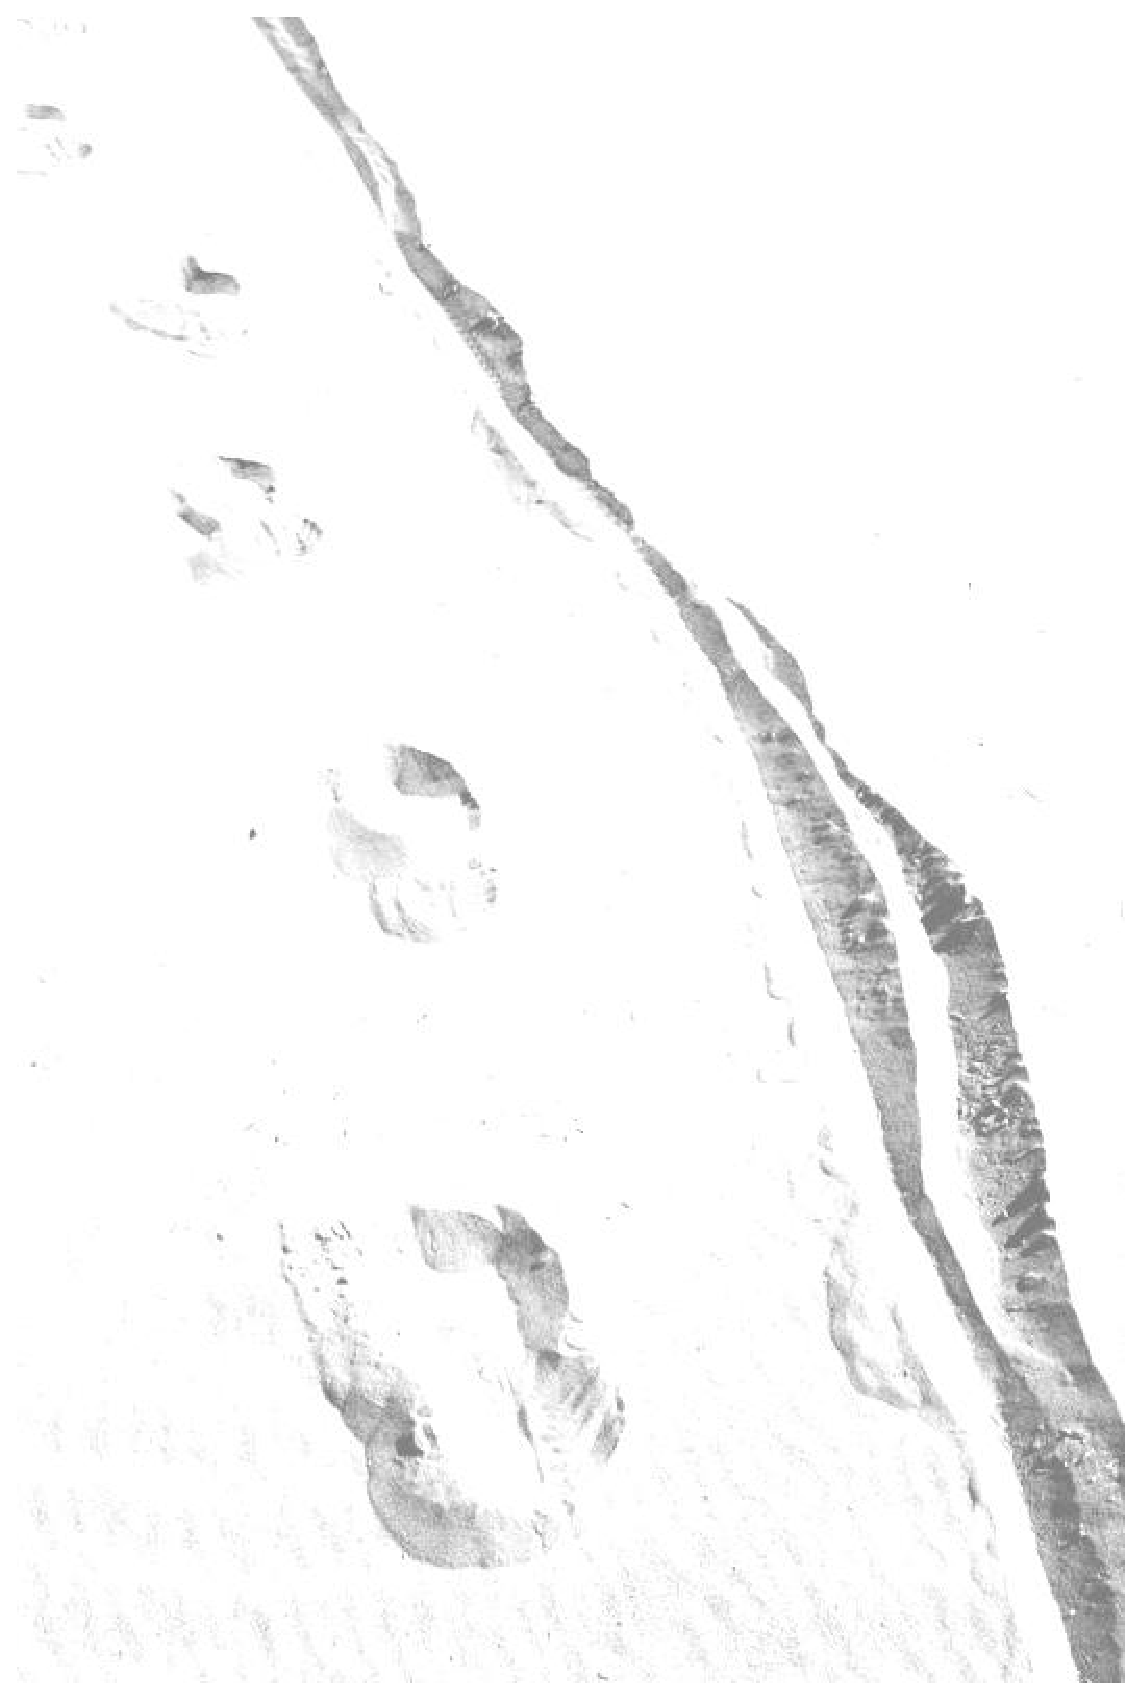
\includegraphics[width=0.55\paperwidth, height = \paperheight]{Figures/Track.eps}}}
  \begin{frame}{\normalsize Outline}
  \tableofcontents[currentsection]
  \end{frame}}
}



\title[AI for Decisions]{AI for Operational Decisions\\ Some perspectives from recent research
}
\author[S. Gros]{\large Prof. Sebastien Gros}
\institute[NTNU]{Department of Cybernetic \\ Faculty of Information Technology \\  NTNU}
\date[Fall 2025]{Freiburg PhD School}

%%%%%%%%%%%%%%%%%%%%%%%%%%%%%%%%%%%%%%%%%%%%%%%%%%%%%%%%%%%%%%%%%%%%%%%%

\begin{document}












\begin{frame}{\normalsize Orientation}
\textbf{What we have seen:} 
\begin{itemize}
\footnotesize
\item RLMPC, why does it work \& different flavors
\end{itemize}
\vspace{.5cm}
\visible<2->{
\textbf{What we will do now:} 
\begin{itemize}
\footnotesize
\item The theory is not about MPC, it is about MDPs (MPC is a special case)
\item It has broader implications for AI and model-based decision making
\item Provide (tentative) practical ideas for in Sim2Real
\end{itemize}}
\end{frame} 


{\usebackgroundtemplate{
 \parbox[c][\paperheight][b]{\paperwidth}{
    \flushright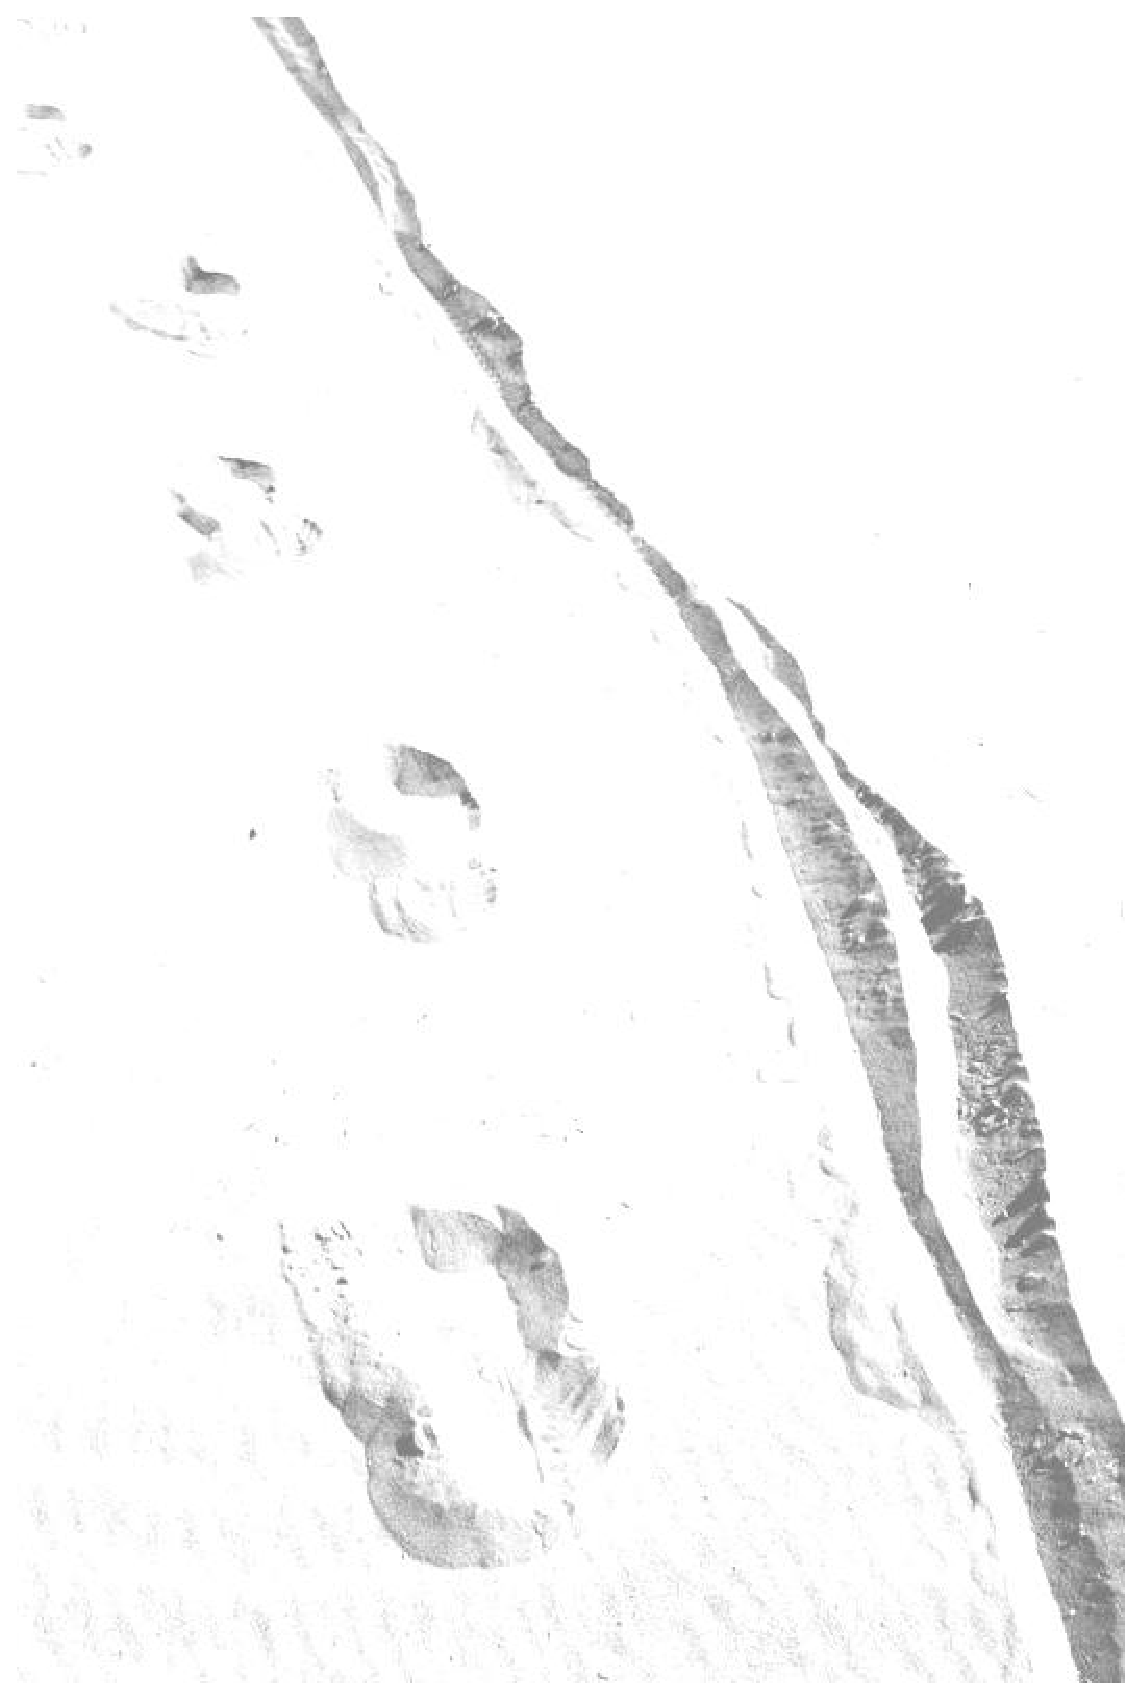
\includegraphics[width=0.55\paperwidth, height = 1\paperheight]{Figures/Track.eps}}}
\begin{frame}
\titlepage
\end{frame}}




%
%\begin{frame}{\normalsize Disclaimer \& Forewords}
%\footnotesize
%\begin{columns}[t]
%\column{0.5\textwidth}
%\textbf{About me} 
%\begin{itemize}
%\item Research in Optimal Control, Markov Decision Processes, Stochastic Optimization, Numerical algorithms, Machine Learning, Reinforcement Learning
%\item Applications in Energy, Energy Economics, Medical Engineering
%\end{itemize}
%
%
%\column{0.5\textwidth}
%\textbf{On this talk}
%\begin{itemize}
%\item This will be a ``high-level" discussion!
%\item Research started in 2018
%\begin{itemize}
%\scriptsize
%\item About 50 papers on the topic
%\item Focused on Reinforcement Learning and MPC, now generalizing
%\end{itemize}
%\item Statistics are underlying everything, great to talk to experts
%\item I will spend time building the background \tiny{(maybe pedestrian, but nothing is ever obvious)}
%\end{itemize}
%\end{columns}
%\vspace{0.25cm}
%\includegraphics[width=1\textwidth,clip]{Figures/SmartGridLab.eps}
%
%\end{frame}

%
%
%\section{Decision making}
%
%\begin{frame}{\normalsize Types of decisions}
%\footnotesize
%\vspace{-.5cm}
%\begin{center}
%\textbf{Focus of this talk is on sequential decision making}
%\end{center}
%\vspace{-.25cm}
%\begin{columns}
%\column{0.7\textwidth}
%\visible<2->{
%\begin{itemize}
%\item At every (discrete) time instant
%\begin{itemize}
%\scriptsize
%\item new information is available
%\item decide of a new action to take on the environment
%\end{itemize}
%\item Information is measurements, forecasts, known future
%\item Rational utility to maximize, guiding the decisions
%\item Actions have ``long-term consequences" on performance
%\item Policy $\vect\pi$ is a function from information  to action
%\item Reality is assumed stochastic
%\end{itemize}
%}
%
%\column{0.3\textwidth}
%
%
%\newcommand{\Sys}{\vspace{-0.25cm}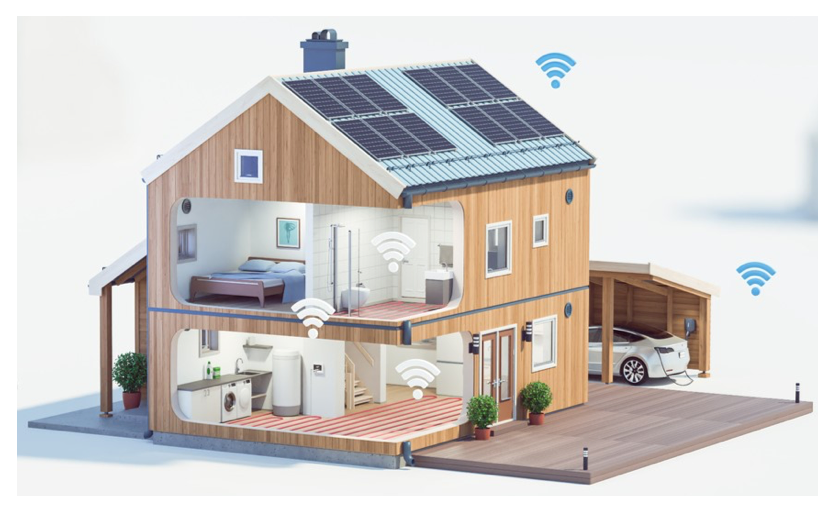
\includegraphics[width=1\textwidth,clip]{Figures/SmartHouse.eps}}
%
%\tikzstyle{Sys_block} = [rectangle, draw, fill=none,  text width=3.cm, text centered, rounded corners, minimum height=4em,inner sep=2pt]
%\tikzstyle{Opt_block} = [rectangle, draw, fill=myLightGreen,  text width=3cm,  text centered, rounded corners]
%\tikzstyle{line} = [draw, -latex']
%
%\begin{tikzpicture}[->,>=stealth']
%
%\node [Sys_block] (sys0) {\Sys};
%
% 
%
% \node [Opt_block, below of=sys0, node distance = 2.7cm] (opt0) {
% \begin{minipage}[c]{3cm}
% \center
%\textbf{Policy} $\vect\pi$\\
%Information to Action
%\end{minipage}
% };
% 
% \path  (sys0) edge[bend left=20]  node[anchor=west] {Information} (opt0)
% (opt0) edge[bend left=20]  node[anchor=east] {Action} (sys0);
%\end{tikzpicture}
%\end{columns}
%
%\vspace{.25cm}
%\visible<3->{
%\textcolor{myBlue2}{\textbf{Ubiquitous problem in our society}}, e.g.
%\begin{itemize}
%\scriptsize
%\item Process control: max revenues, min emissions and wastes / decide on flows, volumes, temperatures
%\item Energy management: min cost of energy / decide on biddings 
%\item Digital healthcare: maximize quality / decide on treatments, clinical pathways
%\item etc.
%\end{itemize}
%}
%
%\visible<4->{\center
%\textbf{Framework to discuss that problem is \textcolor{myRed2}{Markov Decision Processes}}} 
%
%\end{frame}
%
%
%
\section{Decisions from data}
%
%\begin{frame}{\normalsize Markov Decision Processes (MDP)}
%\footnotesize
%\vspace{-.5cm}
%\begin{columns}[t]
%\column{0.49\textwidth}
%\begin{block}{}
%\center
%\textbf{Stochastic state transitions}
%$$\vect s,\vect a\rightarrow \vect s_+$$
%(state-action $\rightarrow$ next state)
%\end{block}
%
%
%
%\column{0.49\textwidth}
%\begin{block}{}
%\center
%\textbf{Utility function} 
%$L(\vect s,\vect a)\in \mathbb R$
%\begin{itemize}
%\item Instantaneous performance
%\item $\infty$ if constraints are violated
%\end{itemize}
%\end{block}
%
%\end{columns}
%
%\begin{columns}[t]
%\column{0.45\textwidth}
%\begin{itemize}
%\item \visible<2->{\textbf{Policy}
%$$\vect a = \vect\pi(\vect s)$$ 
%is how we act on the system}
%\item \visible<3->{ \textbf{Closed-loop performance} 
%\begin{align*}
%J\left(\vect \pi\right) = \mathbb E\left[\left.\sum_{k=0}^\infty \gamma^kL\left(\vect s_k,\vect a_k\right)\,\right|\, \vect a_k = \vect\pi(\vect s_k) \right]
%\end{align*}
%with discount $\gamma \in [0,1]$}
%\item  \visible<4->{ \textbf{Optimal policy}: $\vect \pi^\star$ from
%$$\min_{\vect \pi}\,J\left(\vect \pi\right)$$}
%\end{itemize}
%
%\column{0.45\textwidth}
%
%
%\vspace{-1cm}
%
%%\begin{overlayarea}{\textwidth}{0.25\textheight}
%%\only<1-15>{
%\begin{figure}
%\newcommand{\FS}{.8}
%\begin{overlayarea}{\textwidth}{.4\textheight}
%\only<5>{\includegraphics[width=\FS\textwidth,clip]{Figures/SimpleTrajectories1.eps}}
%\only<6>{\includegraphics[width=\FS\textwidth,clip]{Figures/SimpleTrajectories2.eps}}
%\only<7>{\includegraphics[width=\FS\textwidth,clip]{Figures/SimpleTrajectories3.eps}}
%\only<8>{\includegraphics[width=\FS\textwidth,clip]{Figures/SimpleTrajectories4.eps}}
%\only<9>{\includegraphics[width=\FS\textwidth,clip]{Figures/SimpleTrajectories5.eps}}
%\only<10>{\includegraphics[width=\FS\textwidth,clip]{Figures/SimpleTrajectories6.eps}}
%\only<11>{\includegraphics[width=\FS\textwidth,clip]{Figures/SimpleTrajectories7.eps}}
%\only<12>{\includegraphics[width=\FS\textwidth,clip]{Figures/SimpleTrajectories8.eps}}
%\only<13>{\includegraphics[width=\FS\textwidth,clip]{Figures/SimpleTrajectories9.eps}}
%\only<14>{\includegraphics[width=\FS\textwidth,clip]{Figures/SimpleTrajectories10.eps}}
%\only<15->{\includegraphics[width=\FS\textwidth,clip]{Figures/SimpleTrajectories11.eps}}
%\end{overlayarea}
%\end{figure}
%%}
%\visible<16->{
%\begin{alertblock}{}
%\center
%Decisions at time $k$ taken based on current information $\vect s_k$, knowing that the future is uncertain, and that more information will be available for subsequent decisions
%\end{alertblock}
%}
%%\end{overlayarea}
%
%
%\end{columns}
%
%\end{frame}
%
%\end{document}
%
%
%\begin{frame}{\normalsize Policy from repeated planning (MPC)}
%\footnotesize
%\vspace{-.45cm}
%\begin{center}
%\textbf{Optimize a plan over finite horizon, apply first action, repeat}
%\end{center}
%\vspace{-.75cm}
%\begin{columns}[t]
%\column{0.4\textwidth}
%\begin{block}{}
%\textbf{MPC}: at {\color{blue}current state $\vect s$}
%\vspace{-.5cm}\\
%
%\begin{align*}
%\min_{\vect x,{\color{myGreen3}\vect u}}&\quad  T\left(\vect x_N\right) + \sum_{k=0}^{N-1}\gamma^k L\left(\vect x_k,\vect u_k\right)  \\
%\mathrm{s.t.}&\quad \vect x_{k+1} = \vect f\left(\vect x_k,\vect u_k\right)\\
%%&\quad  \vect h\left(\vect x_k,\vect u_k\right)\leq 0\\
%&\quad \vect{x}_0 = {\color{blue}\vect s}
%\end{align*}
%apply {\color{myGreen3}action $\vect a = \vect u_0^\star$} to the system
%%policy $\vect\pi^\mathrm{MPC}\left(\vect s\right) = {\color{myGreen3}\vect u^\star_{0}}$
%\end{block}
%
%\column{0.6\textwidth}
%\vspace{-.2cm}
%\begin{figure}
%\newcommand{\FS}{.8}
%\begin{overlayarea}{\textwidth}{0.45\textheight}
%\only<1>{\includegraphics[width=\FS\textwidth,clip]{Figures/MPC0.eps}}
%\only<2>{\includegraphics[width=\FS\textwidth,clip]{Figures/MPC1.eps}}
%\only<3>{\includegraphics[width=\FS\textwidth,clip]{Figures/MPC2.eps}}
%\only<4>{\includegraphics[width=\FS\textwidth,clip]{Figures/MPC3.eps}}
%\only<5>{\includegraphics[width=\FS\textwidth,clip]{Figures/MPC4.eps}}
%\only<6>{\includegraphics[width=\FS\textwidth,clip]{Figures/MPC5.eps}}
%\only<7>{\includegraphics[width=\FS\textwidth,clip]{Figures/MPC6.eps}}
%\only<8->{\includegraphics[width=\FS\textwidth,clip]{Figures/MPC7.eps}}
%\end{overlayarea}
%\end{figure}
%\end{columns}
%
%\vspace{.1cm}
%
%\begin{columns}
%\column{0.45\textwidth}
%\visible<9->{
%\begin{block}{}
%\textbf{MPC} 
%\begin{itemize}
%\item is \textbf{based on planning} the future
%\item  \textbf{Policy} from repeated planning $$\vect\pi^\mathrm{MPC}\left(\vect s\right) = {\color{myGreen3}\vect u^\star_{0}}$$
%\end{itemize}}
%\end{block}
%
%\column{0.5\textwidth}
%
%\visible<10->{
%\begin{alertblock}{}
%\textbf{Repeated planning (MPC)}
%\begin{itemize}
%\item Builds a policy for the cost of planning 
%\item Complex relationship \\ ``optimal plan" $\leftrightarrow$ ``optimal policy" 
%\item Stochastic versions exist
%\end{itemize}
%
%\end{alertblock}
%}
%
%\end{columns}
%\visible<11->{
%\center
%\textbf{We will get back to that...}
%}
%
%
%\end{frame}
%
%





\begin{frame}{\normalsize Model-Free Pathway - ``Pure" Reinforcement Learning}
\footnotesize

\newcommand{\Sys}{\vspace{-0.25cm}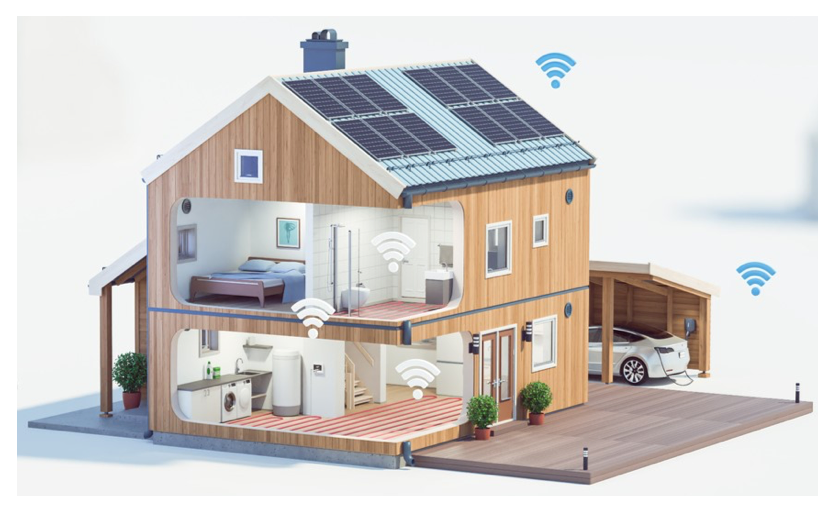
\includegraphics[width=1\textwidth,clip]{Figures/SmartHouse.eps}}

\tikzstyle{Sys_block} = [rectangle, draw, fill=none,  text width=3.cm, text centered, rounded corners, minimum height=4em,inner sep=2pt]
\tikzstyle{Opt_block} = [rectangle, draw, fill=myLightGreen,  text width=3cm,  text centered, rounded corners]
\tikzstyle{RL_block} = [rectangle, draw, fill=myLightBlue,  text width=2.75cm, text centered, rounded corners]    
\tikzstyle{line} = [draw, -latex']

\begin{columns}[t]
\column{0.6\textwidth}



\begin{tikzpicture}[->,>=stealth']

\node [Sys_block] (sys0) {\Sys};

  \visible<2->{
\node [RL_block, left of=sys0, node distance = 4.75cm] (RL0) {
 \begin{minipage}[c]{2.75cm}
\textbf{RL} estimates
\begin{align*}
\nabla_{\vect\theta}J\left(\vect\pi_{\vect \theta}\right)
\end{align*}
\flushright from data
\end{minipage}
 };}
 

 \node [Opt_block, below of=sys0, node distance = 2.7cm] (opt0) {
 \begin{minipage}[c]{3cm}
 \center
\textbf{Policy}
 \vspace{-0.1cm}
\begin{align*}
\vect a = \vect\pi_{\vect \theta}(\vect{s})
\end{align*}

\end{minipage}
 };
 
 
 \path  (sys0) edge[bend left=20]  node[anchor=west] {State} (opt0)
 (opt0) edge[bend left=20]  node[anchor=east] {Actions} (sys0);
 \visible<2->{ \path  (sys0) edge  node[anchor=south] {Real Data} (RL0);}
 \visible<3->{  \path  (RL0) edge[bend right=20]  node[anchor=north east,xshift=0em] {$\vect\theta\leftarrow \vect\theta-\alpha\nabla_{\vect\theta}J\left(\vect\pi_{\vect \theta}\right)$ } (opt0);}
\end{tikzpicture}


\column{0.375\textwidth}
\begin{itemize}
\item Define policy $\vect\pi_{\vect \theta}$ as a parametrized function 
\item Optimize policy as:
\begin{equation*}
\min_{\vect\theta}\,\, J\left(\vect\pi_{\vect \theta}\right)
\end{equation*}
%\item \visible<2->{$\nabla_{\vect\theta}J\left(\vect\pi_{\vect \theta}\right)$ can be estimated from data}
\item \visible<3->{Gradient descent can be used to optimize policy}
\end{itemize} 
\end{columns}
\vspace{.5cm}
 \visible<4->{
\textbf{Remarks}
\begin{itemize}
\item $\vect\pi_{\vect \theta}(\vect{s})$ often from DNN
\item End-to-end training requires a lot of data and effort
\item Difficult to provide explainability and guarantees on the policy we obtain
\item Poor track record of industrial adoption (exception chatbots)
%, generate artificial data that ``look like" reality, etc.
\end{itemize}}
 \visible<5->{\flushright $\rightarrow$policy is often trained on \textcolor{myBlue2}{\textbf{high-fidelity simulations}}: embed knowledge, reduce costs, manage safety, promote explainability, control the training
}

\end{frame}



%\begin{frame}{\normalsize Predictive AI Models}
%\footnotesize
%\begin{center}
%\textbf{``Any tool" turning data into predictions on how reality will evolve}\\ {\scriptsize(My definition, big stretch, I know...)}\\\vspace{.5cm} 
%\textbf{
%\textcolor{myBlue2}{My point will not so much on how we predict but ``what" we predict}
%}
%\end{center}
%
%
%
%\begin{columns}[t]
%\column{0.5\textwidth}
%
%\visible<2->{
%\textbf{Applies to}
%\begin{itemize}
%\item Classic AI tools {\tiny(DNN, LSTM, TFT, etc)}
%\item Statistics of time series
%\item Hybrid modelling
%\item Linear predictors
%\item etc.
%\end{itemize}}
%
%\column{0.5\textwidth}
%
%\visible<3->{
%\textbf{Deliver}
%\begin{itemize}
%\item Probabilistic predictions, e.g.
%\begin{itemize}
%\scriptsize
%\item sampling-based 
%\item scenarios
%\item approximate distribution
%\end{itemize}
%\item Deterministic predictions
%\begin{itemize}
%\scriptsize
%\item distill statistics in ``single-point"
%\item expected value, MLE, etc
%\end{itemize}
%\end{itemize}}
%\end{columns}
%
%
%\end{frame}


\begin{frame}{\normalsize Model-based Pathway - Predictive AI Models \scriptsize{(data-driven, ML, etc)}}
\footnotesize
\vspace{-0.25cm}
\begin{columns}
\column{0.4\textwidth}
\visible<2->{
\begin{block}{\scriptsize One-step model}
\textbf{AI model} e.g.
\vspace{-0.1cm}
\begin{align*}
\hat{\vect{s}}_{k+1} \sim  \rho_{\vect{\theta}}(\cdot\,|\,\vect{s}_k,\vect{a}_k)
\end{align*}
\vspace{-0.75cm}
\flushright fitting data %$\rho$ 
\end{block}
}



\column{0.55\textwidth}
\begin{overlayarea}{\textwidth}{.3\textheight}
\only<1-3>{
\vspace{.4cm} 
\textbf{Real world}: ${\vect{s}}_{k+1} \sim  \rho(\cdot\,|\,\vect{s}_k,\vect{a}_k)$
\vspace{-0.1cm}
\begin{itemize}
\item Data with enough ``richness" 
\end{itemize} 


%\begin{figure}
%\newcommand{\FS}{.8}
%\psfrag{x0}[Bl][Bl][1]{$\vect{s}_k$}
%\psfrag{t}[Bl][Bl][.7]{Time}
%\psfrag{P}[Bl][Bl][1]{$\rho_{\vect\theta}$}
%%\includegraphics[width=\FS\textwidth,clip]{Figures/StatePropagationStochastic.eps}
%\includegraphics[width=\FS\textwidth,clip]{Figures/StatePropagation.eps}
%\end{figure}

}
\only<4->{
\begin{alertblock}{}
\center
Virtual data from ``simulating" $\hat{\vect{s}}_{k+1} \sim  \rho_{\vect{\theta}}(\cdot\,|\,\vect{s}_k,\vect{a}_k)$ forward (Monte Carlo)
\end{alertblock}
\vspace{-.25cm}
}
\visible<5->{
\begin{alertblock}{}
\center
In most cases, $\rho_{\vect{\theta}}$ is a fairly simple representation of reality $\rho$, easy to sample from
\end{alertblock}
 }
\end{overlayarea}


\end{columns}
\vspace{-.2cm}
\visible<2->{
\begin{center}
\textit{Here we no longer need the model $\rho_{\vect{\theta}}$ to be ``optimization-friendly"}
\end{center}
}
%\vspace{.2cm}
%\begin{overlayarea}{\textwidth}{.5\textheight}
%\only<3-5>{
\visible<3->{
\textbf{Model parameters $\vect\theta$}
\begin{itemize}
\item Selected such that model $\rho_{\vect{\theta}}$ ``ressembles" reality $\rho$, using data (+ physics)
\item Deterministic models are a special case of $\rho_{\vect{\theta}}$
\item Many methods, from Least Squares and MLE to Bayesian and Adversarial Learning
\item Still, in most cases $\rho_{\vect{\theta}}$ ``simplifies" $\rho$ because
\begin{itemize}
\scriptsize
\item need for huge amounts of data to decide $\vect\theta$ if model is very rich
\item computationally demanding simulations if $\rho_{\vect{\theta}}$ is expensive to sample from
\end{itemize}
\item Then
\begin{itemize}
\scriptsize
\item biases in case of insufficiently rich model structure
\item validity is limited to some parts of the state-action space
\item only few first moments are correct (typ. mean + variance)
\end{itemize}
\end{itemize}}


\end{frame}


\begin{frame}{\normalsize Back to MPC - A ``Classical" View on Decision Making}
\footnotesize
\begin{columns}
\column{0.45\textwidth}
\begin{block}{}
\textbf{Policy} $\vect\pi_{\vect \theta}(\vect{s})$ given implicitly by 
\vspace{-.5cm}\\
\begin{align*}
\min_{\vect x,{\color{myGreen3}\vect u}}&\quad  \mathbb E\left[ T\left(\vect x_N\right) + \sum_{k=0}^{N-1} L\left(\vect x_k,\vect u_k\right) \right] \\
\mathrm{s.t.}&\quad \vect x_{k+1} \sim \rho_{\vect\theta}\left(\vect x_k,\vect u_k\right)\\
%&\quad  \vect h\left(\vect x_k,\vect u_k\right)\leq 0\\
&\quad \vect{x}_0 = {\color{blue}\vect s}
\end{align*}
\flushright use $\vect\pi_{\vect \theta}(\vect{s}) = {\color{myGreen3}\vect u_0^\star}$ on the system
\end{block}

\column{0.525\textwidth}
\vspace{-0.3cm}
\begin{overlayarea}{\textwidth}{0.3\textheight}
\only<3>{
\begin{alertblock}{}
\textbf{\textcolor{black}{Defines a paradigm}}...\\
\vspace{0.1cm}
\begin{itemize}
\item Performance from model accuracy
$$\text{i.e. }\rho_{\vect\theta}\text{ ``close enough" to }\rho$$
\item ``Ignore" that we replan all the time
\end{itemize}
\end{alertblock}
}
\only<4->{

\textbf{Relationship $\vect\pi_{\vect\theta}$ to $\vect\pi^\star$??}
\begin{itemize}
\scriptsize
\item They match if $\rho_{\vect{\theta}}$ is exact and deterministic
\item But it usually cannot be...
\end{itemize}
 \vspace{-0.3cm}
\visible<5->{
\begin{alertblock}{}
\center\textbf{
``Standard methods" for choosing $\vect \theta$ in general do not yield the best $\vect\pi_{\vect \theta}$.\\
RL over MPC can fix that, $L$ becomes part of the model}
\end{alertblock}
}}
\end{overlayarea}




\end{columns}

\newcommand{\Sys}{\vspace{-0.25cm}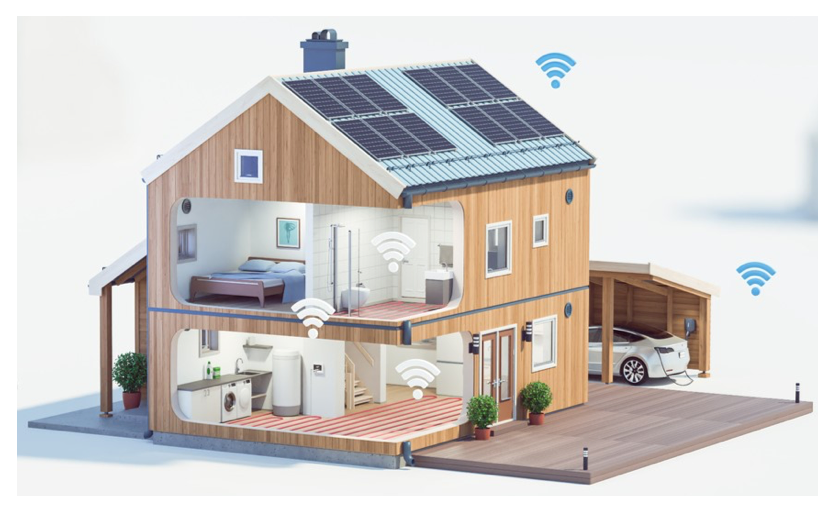
\includegraphics[width=1\textwidth,clip]{Figures/SmartHouse.eps}}

\tikzstyle{Sys_block} = [rectangle, draw, fill=none,  text width=3.cm, text centered, rounded corners, minimum height=4em,inner sep=2pt]
\tikzstyle{Opt_block} = [rectangle, draw, fill=myLightGreen,  text width=2.85cm,  text centered, rounded corners]
\tikzstyle{ID_block} = [rectangle, draw, fill=myLightBlue,  text width=3cm, text centered, rounded corners]    
\tikzstyle{line} = [draw, -latex']

\begin{tikzpicture}%[node distance = 4cm, auto]

\node [Sys_block] (sys0) {\Sys};
\node [Opt_block, left of=sys0, node distance = 4cm] (opt0) {
 \begin{minipage}[c]{2.75cm}
 \center
\textbf{MPC policy}
 \vspace{-0.1cm}
\begin{align*}
\vect\pi_{\vect \theta}(\vect{s})
\end{align*}
\textbf{from model}
\begin{align*}
\vect{s}_{k+1} \sim {\rho}_{\vect{\theta}}(.\,|\,\vect{s}_k,\vect{a}_k)
\end{align*}
\end{minipage}
 };
 
\visible<2->{
\node [ID_block, right of=sys0, node distance = 4.75cm] (ID0) {
 \begin{minipage}[c]{3cm}
\textbf{AI model} 
\begin{align*}
\hat{\vect{s}}_{+} \sim \rho_{\vect{\theta}}\left(\cdot\,|\,\vect{s},\vect{a}\right)
\end{align*}
\vspace{-.75cm}
\flushright fitting data $\rho$
\end{minipage}
 };
%\node [ID_block, right of=sys0, node distance = 4.5cm] (ID0) {
% \begin{minipage}[c]{3.0cm}
%\center
%\textbf{AI model} adjust ${\vect{\theta}}$ to fit model ${\rho}_{\vect{\theta}}$ to data $\vect{s}_k,\vect{a}_k,\vect{s}_{k+1}$
%\end{minipage}
% }; 
 }
\path [line] (opt0) -- node [ anchor=south] {$\vect{a}$} (sys0);
\path [line] (sys0.south)  -- ++(0,-0.5) -| node [ anchor=north] {$\vect{s}$} (opt0.south);
\visible<2->{\path [line] (sys0) -- node [ anchor=center,xshift=-.5em] { \begin{minipage}[c]{1cm}
  \center
 Data\\ knowledge
 \end{minipage}} (ID0);}
\visible<2->{\path [line] (ID0.north) -- ++(0,0.6) -| node [ anchor=south] {${\vect{\theta}}$} (opt0.north);}
 \end{tikzpicture}
 \vspace{-.25cm}
\center
\visible<6->{\textbf{This is not the only way of taking decisions from models}}
\end{frame}




\begin{frame}{\normalsize Decision policy from AI models (Sim2Real)}
\footnotesize


\newcommand{\Sys}{\vspace{-0.25cm}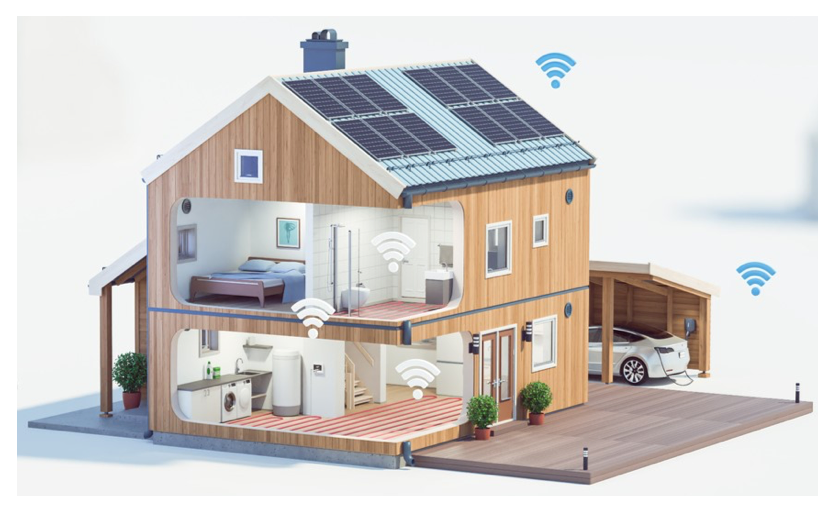
\includegraphics[width=1\textwidth,clip]{Figures/SmartHouse.eps}}

\tikzstyle{Sys_block} = [rectangle, draw, fill=none,  text width=3.cm, text centered, rounded corners, minimum height=4em,inner sep=2pt]
\tikzstyle{Obj_block} = [rectangle, draw, fill=myLightRed,  text width=2.7cm, text centered, rounded corners, minimum height=4em,inner sep=2pt]
\tikzstyle{Opt_block} = [rectangle, draw, fill=myLightGreen,  text width=3cm,  text centered, rounded corners]
\tikzstyle{ID_block} = [rectangle, draw, fill=myLightBlue,  text width=3cm, text centered, rounded corners]    
\tikzstyle{line} = [draw, -latex']

\begin{tikzpicture}[->,>=stealth']

\node [Sys_block] (sys0) {\Sys};

\node [ID_block, left of=sys0, node distance = 5cm] (ID0) {
 \begin{minipage}[c]{3cm}
\textbf{AI model} 
\begin{align*}
\hat{\vect{s}}_{+} \sim \rho_{\vect{\theta}}\left(\cdot\,|\,\vect{s},\vect{a}\right)
\end{align*}
\vspace{-.75cm}
\flushright fitting data $\rho$
\end{minipage}
 };


 \visible<2->{
 \node [Opt_block, below of=ID0, node distance = 2.5cm] (opt0) {
 \begin{minipage}[c]{3cm}
 \center
\textbf{Policy}
 \vspace{-0.2cm}\\
 \begin{overlayarea}{\textwidth}{0.1\textheight}
\only<1-4>{
 \vspace{-0.2cm}
\begin{align*}
\vect a=\vect \pi_{\vect \nu}(\vect{s})
\end{align*}
}
\only<5->{
 \vspace{-0.2cm}
\begin{align*}
\vect a=\vect \pi_{\vect \theta}(\vect{s})
\end{align*}}
\end{overlayarea}
optimal for AI model
\end{minipage}
 };}
 
 \visible<2->{
 \node [Obj_block, left of=opt0, node distance = 4cm] (Obj0) {
 \begin{minipage}[c]{2.7cm}
\textbf{Objective}
\vspace{-.5cm}\\
\begin{align*}
L\left(\vect s,\vect a\right)
\end{align*}
\vspace{-0.8cm}
\flushright possibly unbounded
\end{minipage}
 };}
 
 \path 
 (sys0) edge  node[anchor=center,xshift=-.5em] {
  \begin{minipage}[c]{1cm}
  \center
 Data\\ knowledge
 \end{minipage}} (ID0);
 
\visible<2->{ \path  (ID0) edge[bend left=20]  node[anchor=west] {Virtual data} (opt0);}
\visible<2->{ \path   (opt0) edge[bend left=20]  node[anchor=east] {Actions} (ID0);}
\visible<3->{ \path  (opt0) edge[bend right=20]  node[anchor=west,xshift=1em] {Policy} (sys0);}
\visible<2->{ \path  (Obj0) edge  node[anchor=south] {Cost} (opt0) ;}
\end{tikzpicture}



\begin{overlayarea}{\textwidth}{0.45\textheight}
\only<1-4>{\visible<1-4>{
\vspace{-.25cm}
\textbf{Classical Process:}}
\begin{itemize}
\item \visible<1-4>{Fit AI model $\rho_{\vect\theta}$ to real data}
\item \visible<2-4>{Develop optimal policy for $L$ and $\rho_{\vect\theta}$ from AI model, e.g. using In-Sim RL
\begin{itemize}
\scriptsize
\item Define parametrized policy $\vect\pi_{\vect\nu}$
\item Optimize policy parameters $\vect\nu$ for performance w.r.t. AI model: $\rho_{\vect\theta},L\,\rightarrow\,\vect\nu^\star$
\end{itemize}}
\item \visible<3-4>{Transfer policy $\vect\pi_{\vect\nu^\star}$ into the real world}
\end{itemize}
%\vspace{-.4cm}
\center
\visible<4>{\textbf{Note: policy parameters $\vect\nu^\star$ optimal for AI model become function of $\vect\theta$ \\ Let's then label $\vect\pi_{\vect\theta} = \vect\pi_{\vect\nu^\star}$ for simplicity}}
}
\only<5->{
\textbf{Remarks}
\begin{itemize}
\scriptsize
\item Relationship $\vect\pi_{\vect\theta}$ to $\vect\pi^\star$??
\begin{itemize}
\scriptsize
\item They match if $\rho_{\vect{\theta}}=\rho$, i.e. if model is exact
\item But $\rho_{\vect{\theta}}$ is (almost always) an approximation
\end{itemize}
\end{itemize}}
 \vspace{-0.3cm}
\visible<6->{
\begin{alertblock}{}
\center
\textbf{Are ``standard methods" for choosing $\vect \theta$ resulting in a good policy $\vect\pi_{\vect \theta}$?? Empirically the answer is ``no". Then how to choose $\vect \theta$ to get a good policy?}
\end{alertblock}
}


\end{overlayarea}

\end{frame}

\begin{frame}{\normalsize MPC or Sim2Real - It's the same question...}
\footnotesize
\vspace{-.1cm}
\visible<2->{
\begin{center}
\textit{The theory is about model-based decisions, and equivalences between MDPs}
\end{center}}
\vspace{-.6cm}
\begin{columns}[t]
\column{0.49\textwidth}
\visible<3->{
\begin{block}{\footnotesize \textcolor{myRed}{World} \textcolor{black}{MDP}}
\textbf{World MDP definition} 
\begin{itemize}
\item States $\vect s$ and actions $\vect a$
\item Cost $\textcolor{myRed}{L}\left(\vect s,\vect a\right)$
\item Transition $\vect s_+\sim\textcolor{myRed}{\rho}\left[\,\cdot\,|\vect s,\vect a\right]$
\end{itemize}
\visible<4->{
\textbf{Optimal value functions}
\vspace{-.1cm}
\begin{align*}
V^\star\left(\vect s\right) &= \min_{\vect a}\,Q^\star\left(\vect s,\vect a\right) \\
Q^\star\left(\vect s,\vect a\right)&= \textcolor{myRed}{L}\left(\vect s,\vect a\right)+\gamma \mathbb E_{\vect s_+\sim\textcolor{myRed}{\rho}}\left[V^\star\left(\vect s_+\right)|\vect s,\vect a\right]\\
\end{align*}}
\vspace{-1cm}\\
\visible<5->{
\textbf{Optimal policy}
\vspace{-0.2cm}
\begin{align*}
\vect\pi^\star\left(\vect s\right)=\argmin_{\vect a}\,Q^\star\left(\vect s,\vect a\right)
\end{align*}}
\vspace{-.4cm}
\end{block}}
\column{0.001\textwidth}
\column{0.49\textwidth}
\visible<6->{
\begin{block}{\footnotesize \textcolor{myBlue2}{Model} \textcolor{black}{MDP (simulation environment)}}
\textbf{Model MDP definition} 
\begin{itemize}
\item States $\vect s$ and actions $\vect a$
\item Cost $\textcolor{myBlue2}{\hat L}\left(\vect s,\vect a\right)$
\item Transition $\vect s_+\sim\textcolor{myBlue2}{\hat \rho}\left[\,\cdot\,|\vect s,\vect a\right]$
\end{itemize}
\visible<6->{
\textbf{Optimal value functions}
\vspace{-.1cm}
\begin{align*}
\hat V^\star\left(\vect s\right) &= \min_{\vect a}\,\hat Q^\star\left(\vect s,\vect a\right) \\
\hat Q^\star\left(\vect s,\vect a\right)&= \textcolor{myBlue2}{\hat L}\left(\vect s,\vect a\right)+\gamma \mathbb E_{\vect s_+\sim\textcolor{myBlue2}{\hat\rho}}\left[\left.\,V^\star\left(\hat{\vect s}_+\right)\right|\,\vect s,\vect a\right]\\
\end{align*}}
\vspace{-1cm}\\
\visible<6->{
\textbf{Optimal policy}
\vspace{-0.2cm}
\begin{align*}
\hat{\vect\pi}^\star\left(\vect s\right)=\argmin_{\vect a}\,\hat Q^\star\left(\vect s,\vect a\right)
\end{align*}}
\vspace{-.4cm}
\end{block}}
\end{columns}
\visible<7->{
\begin{alertblock}{}
\vspace{-.1cm}
\center \textbf{Theory says} that - under some technical conditions - there is a $\textcolor{myBlue2}{\hat L}$ such that $\hat Q^\star = Q^\star$
\end{alertblock}}
\visible<8->{
\underline{Proof}: telescopic sum, some non-trivial assumptions to prevent $\infty-\infty$ cancellations}
\end{frame}


\begin{frame}{\normalsize More on MDP Equivalence}
\footnotesize
\vspace{-.25cm}
\begin{columns}[t]
\column{0.49\textwidth}
\begin{block}{\footnotesize \textcolor{myRed}{World} \textcolor{black}{MDP}}
\begin{itemize}
\item States $\vect s$ and actions $\vect a$
\item Cost $\textcolor{myRed}{L}\left(\vect s,\vect a\right)$
\item Transition $\vect s_+\sim\textcolor{myRed}{\rho}\left[\,\cdot\,|\vect s,\vect a\right]$
\end{itemize}
\end{block}
\column{0.001\textwidth}
\column{0.49\textwidth}

\begin{block}{\footnotesize \textcolor{myBlue2}{Model} \textcolor{black}{MDP}}
\begin{itemize}
\item States $\vect s$ and actions $\vect a$
\item Cost $\textcolor{myBlue2}{\hat L}\left(\vect s,\vect a\right)$
\item Transition $\vect s_+\sim\textcolor{myBlue2}{\hat \rho}\left[\,\cdot\,|\vect s,\vect a\right]$
\end{itemize}
\end{block}


\end{columns}

\visible<2->{
\begin{alertblock}{}
\vspace{-.1cm}
\textbf{Theory says} that 
\vspace{-.1cm}
\begin{itemize}
\scriptsize
\item Under some technical conditions there is a $\textcolor{myBlue2}{\hat L}$ such that $\hat Q^\star = Q^\star$
\item \visible<3->{For $\textcolor{myBlue2}{\hat L}=L$ there is a (non-unique) ``optimal" model $\textcolor{myBlue2}{\hat\rho}$ such that $\hat Q^\star = Q^\star$}
\item \visible<4->{Conditions for model $\textcolor{myBlue2}{\hat\rho}$ ``optimality" $\neq$ min of classical loss functions (except. LQR)}
\item \visible<5->{World MDP and Model MDP do not need to use the same discount $\gamma$}
\end{itemize}
\end{alertblock}}
\vspace{.25cm}
\begin{overlayarea}{\textwidth}{0.5\textheight}
\only<6>{
\textbf{In-Sim policy training uses a Model MDP}
\begin{itemize}
\scriptsize
\item Practitioners mostly work on model $\textcolor{myBlue2}{\hat \rho}$, but ``unsure" on how to tune it
\item In the ML communities, people talk about ``value alignment", we are trying to make this ``MDP equivalence" understood
%\item Finite horizon: ok if correct terminal cost
%\item Scenario tree: rough $\textcolor{myGreen2}{\hat \rho}$
\end{itemize}
}
\only<7->{
\vspace{-.5cm}
\begin{columns}
\column{0.725\textwidth}
\textbf{Remarks}
\begin{itemize}
\scriptsize
\item Non-unique optimal model $\textcolor{myBlue2}{\hat \rho}$ leaves room for aligning it to the real world (classical fitting)
\item \visible<8->{If $V^\star$ is continuous and support of $\textcolor{myRed}{\rho}$ is bounded(?) and path-connected, then we can have support $\textcolor{myBlue2}{\hat \rho}$ $\subset$ support of  $\textcolor{myRed}{\rho}$ }
\item \visible<11->{\textit{More simply said}: we can build optimal models $\textcolor{myBlue2}{\hat \rho}$ that make ``plausible" predictions about the real world.}
\end{itemize}
\column{0.275\textwidth}
\begin{overlayarea}{\textwidth}{0.33\textheight}
\only<9>{
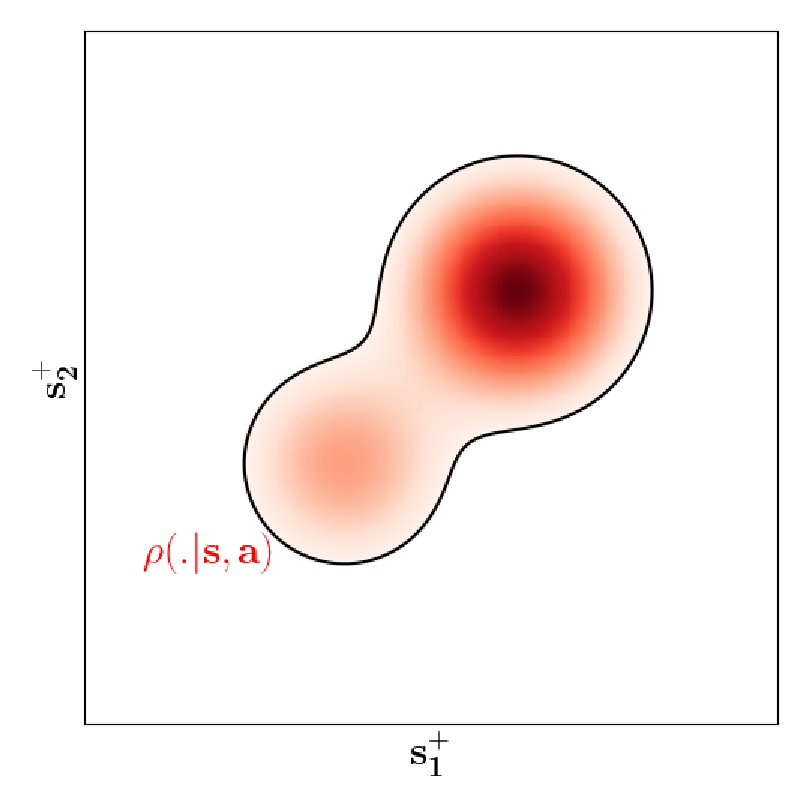
\includegraphics[width=1\textwidth,clip]{Codes/MDPEquivalence/World.eps}
}
\only<10->{
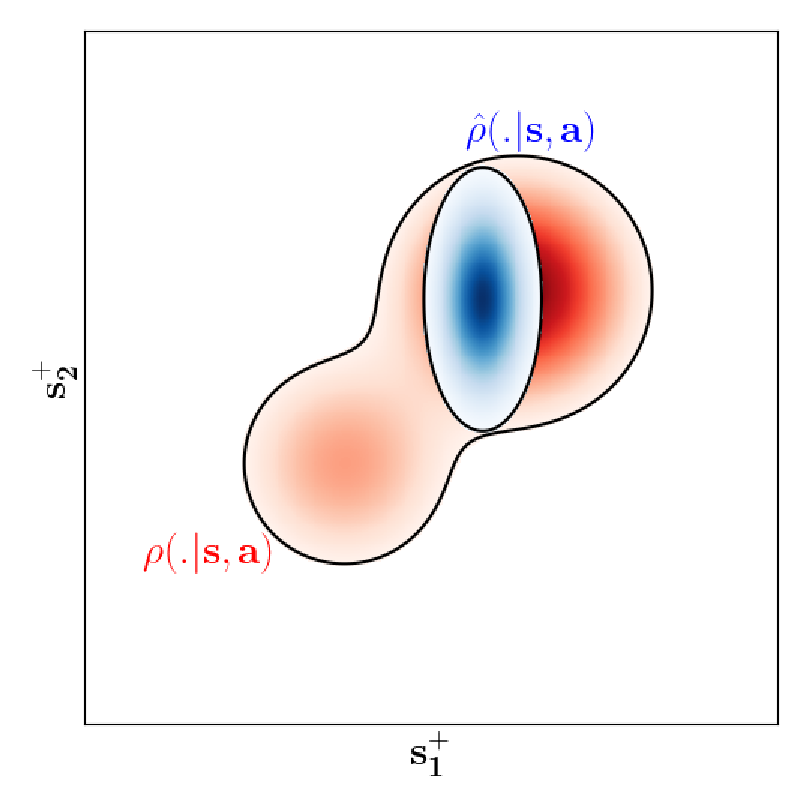
\includegraphics[width=1\textwidth,clip]{Codes/MDPEquivalence/Model.eps}
}
\end{overlayarea}

\end{columns}
}

\end{overlayarea}


\end{frame}
%
%\begin{frame}{\normalsize Is there a catch? A side track...}
%\footnotesize
%\vspace{-1cm}
%\begin{columns}[t]
%\column{0.49\textwidth}
%\begin{block}{\footnotesize \textcolor{myRed}{World} \textcolor{black}{MDP}}
%\begin{itemize}
%\item States $\vect s$ and actions $\vect a$
%\item Cost $\textcolor{myRed}{L}\left(\vect s,\vect a\right)$
%\item Transition $\vect s_+\sim\textcolor{myRed}{\rho}\left[\,\cdot\,|\vect s,\vect a\right]$
%\end{itemize}
%\end{block}
%\column{0.001\textwidth}
%\column{0.49\textwidth}
%
%\begin{block}{\footnotesize \textcolor{myBlue2}{Model} \textcolor{black}{MDP}}
%\begin{itemize}
%\item States $\vect s$ and actions $\vect a$
%\item Cost $\textcolor{myBlue2}{\hat L}\left(\vect s,\vect a\right)$
%\item Transition $\vect s_+\sim\textcolor{myBlue2}{\hat \rho}\left[\,\cdot\,|\vect s,\vect a\right]$
%\end{itemize}
%\end{block}
%
%
%\end{columns}
%\begin{alertblock}{}
%\vspace{-.1cm}
%\center \textbf{Theory says} that - under some technical conditions - there is a $\textcolor{myBlue2}{\hat L}$ such that $\hat Q^\star = Q^\star$
%\end{alertblock}
%\vspace{.25cm}
%\begin{overlayarea}{\textwidth}{0.3\textheight}
%\only<2-4>{
%\textbf{But we are making a strong assumption} (in plain sight)
%\visible<3->{
%\begin{itemize}
%\item Theory assumes that World MDP and Model MDP have the same state $\vect s$
%\item I.e. we need to know the state of the World MDP to build a correct Model MDP
%\item That is often impossible...
%\end{itemize}}
%\flushright\visible<4->{\textbf{The end of a nice theory? No, but it is a word of caution...}}
%}
%\only<5->{\textbf{Eventually the Markov state $\vect s$ boils down to the history of past observations}
%\vspace{-.25cm}
%\begin{flushright}\textit{How to embed that in a model?}\end{flushright}
%\vspace{-.35cm}
%\begin{enumerate}
%\item \visible<6->{``Input-output models": ARX, multi-step predictors (more in a bit), etc.}
%\item \visible<7->{Latent states (a.k.a. embeddings or compressed representations) giving an AI-driven lower-dimensional version of that history}
%\item \visible<8->{State observers giving a model-based lower-dimensional version of that history (more in next slide)}
%\end{enumerate}
% \visible<9->{\center Options 2 and 3 are part of the decision-making process, back-propagate through policy + state ``constructor". }
%}
%\end{overlayarea}
%\end{frame}
%
%\begin{frame}{\normalsize State Estimation in the Learning Loop}
%\footnotesize
%
%\newcommand{\Sys}{\vspace{-0.25cm}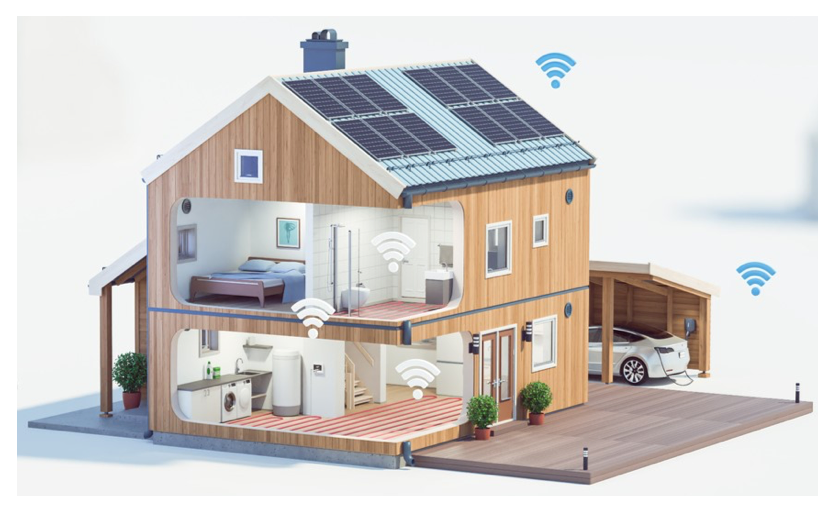
\includegraphics[width=1\textwidth,clip]{Figures/SmartHouse.eps}}
%
%\tikzstyle{Sys_block} = [rectangle, draw, fill=none,  text width=2.5cm, text centered, rounded corners, minimum height=4em,inner sep=2pt]
%\tikzstyle{Opt_block} = [rectangle, draw, fill=myLightGreen,  text width=2cm,  text centered, rounded corners]
%\tikzstyle{ID_block} = [rectangle, draw, fill=myLightBlue,  text width=2.5cm, text centered, rounded corners]    
%\tikzstyle{Obs_block} = [rectangle, draw, fill=myLightRed,  text width=2cm, text centered, rounded corners]    
%\tikzstyle{line} = [draw, -latex']
%
%\begin{tikzpicture}%[node distance = 4cm, auto]
%
%\node [Sys_block] (sys0) {\Sys};
%
%\node [Opt_block, left of=sys0, node distance = 3cm] (opt0) {
% \begin{minipage}[c]{2cm}
% \center
%\textbf{\footnotesize Policy} 
% \vspace{-.1cm}
%$$\vect\pi_{\textcolor{myGreen3}{\vect\theta}}\left({\color{blue}\vect s} \right)$$
%\end{minipage}
% };
%
%\visible<2->{
%\node [Obs_block, below of=opt0, node distance = 1.75cm] (obs0) {
% \begin{minipage}[c]{2cm}
% \center
%\textbf{\footnotesize State estimation} 
% \vspace{-.25cm}
%$${\color{blue}\vect s} = \varphi_{\textcolor{myGreen3}{\vect\theta}}\left(\text{\textcolor{myRed2}{Data}}\right)$$
%%$$\text{Data}\xrightarrow[]{\textcolor{myGreen3}{\vect\theta}} {\color{blue}\vect s}$$
%\end{minipage}
% };
%}
% 
%\node [ID_block, right of=sys0, node distance = 4.2cm] (ID0) {
% \begin{minipage}[c]{2.5cm}
%\textbf{RL} estimates
%\begin{align*}
%\nabla_{\textcolor{myGreen3}{\vect\theta}}J\left(\vect\pi_{\textcolor{myGreen3}{\vect\theta}}\right) 
%\end{align*}
%\flushright from data
%\end{minipage}
% };
% 
%  \visible<3->{
%  \draw[blue,thick] ($(opt0.north east)+(+0.15,0.15)$)  rectangle ($(obs0.south west)+(-0.15,-0.15)$);
%  }
%  
%  
%\path [line] (opt0) -- node [ anchor=south] {$\vect{a}$} (sys0);
%\visible<1>{\path [line] (sys0.south)  -- ++(0,-.5) -| node [ anchor=north] {${\color{blue}\vect s}$} (opt0.south);}
%\path [line] (sys0) -- node [ anchor=south] {\textcolor{myRed2}{Data}} (ID0);
%\path [line] (ID0.north) -- ++(0,0.25) -| node [ anchor=east] {$\textcolor{myGreen3}{\vect\theta}$} (opt0.north);
%
%\visible<2->{\path [line] (sys0.south)   |- node [ anchor=north] {\textcolor{myRed2}{Data}} (obs0.east);}
%\visible<2->{\path [line] (obs0.north)  -- node [ anchor=west] {${\color{blue}\vect s}$} (opt0.south);}
%
%  \visible<3->{
%\path [line] (ID0.south)  -- ++(0,-2) -| node [ anchor=north] {$\textcolor{myGreen3}{\vect\theta}$} (obs0.south);
%  }
%
% \end{tikzpicture}
% 
%
%
%
%
%\begin{columns}
%\column{0.65\textwidth}
%
%\begin{overlayarea}{\textwidth}{0.5\textheight}
%\only<4-6>{
%
%\textbf{Remarks}
%\begin{itemize}
%\scriptsize
%%\item State Estimation (SE) gives ${\color{blue}\vect s} = \varphi_{\textcolor{myGreen3}{\vect\theta}}\left(\text{\textcolor{myRed2}{Data}}\right)$
%\item \visible<4->{Policy is ${\vect\pi}^\text{D}_{\textcolor{myGreen3}{\vect\theta}}\left(\text{\textcolor{myRed2}{Data}}\right) = \vect\pi_{\textcolor{myGreen3}{\vect\theta}}\left(\varphi_{\textcolor{myGreen3}{\vect\theta}}\left(\text{\textcolor{myRed2}{Data}}\right)\right)$}
%\item \visible<5->{Gradient of the policy now is:
%\begin{align*}
%\nabla_{\textcolor{myGreen3}{\vect\theta}} {\vect\pi}^\text{D}_{\textcolor{myGreen3}{\vect\theta}}\left(\text{\textcolor{myRed2}{Data}}\right) = \nabla_{\textcolor{myGreen3}{\vect\theta}}\vect\pi_{\textcolor{myGreen3}{\vect\theta}}\left({\color{blue}\vect s}\right) + \nabla_{\textcolor{myGreen3}{\vect\theta}}\varphi_{\textcolor{myGreen3}{\vect\theta}}\left(\text{\textcolor{myRed2}{Data}}\right) \nabla_{{\color{blue}\vect s}}\vect\pi_{\textcolor{myGreen3}{\vect\theta}}\left({\color{blue}\vect s}\right)
%\end{align*}}
%\vspace{-.5cm}
%\item \visible<6->{Critic is looking at $\text{\textcolor{myRed2}{Data}}\xrightarrow[]{\textcolor{myGreen3}{\vect\theta}} \vect a$, i.e. $Q^{{\vect\pi}^\text{D}_{\textcolor{myGreen3}{\vect\theta}}}\left(\text{\textcolor{myRed2}{Data}},\vect a\right)$}
%\end{itemize}
%
%}
%
%\only<7->{
%\textbf{If $\varphi_{\textcolor{myGreen3}{\vect\theta}}\left(\text{\textcolor{myRed2}{Data}}\right)$ is}
%\begin{itemize}
%\scriptsize
%\item MHE, then its gradient is computed using NLP sensitivities (same as MPC)
%\item DNN, then efficient sensitivity computations exist
%\item Bayesian inference? Belief state? Open research topic...
%\end{itemize}
%}
%
%
%\end{overlayarea}
%
%\column{0.35\textwidth}
%\vspace{-1cm}
%\visible<8->{
%\includegraphics[width=1\textwidth,clip,trim= 0 0 0 0]{Figures/RL_BL_TD}
%}
%
%
%\end{columns}
%
%
%	
%
%
%\end{frame}
%
%\begin{frame}{\normalsize Multi-Step Predictive Control}%: RL for Data-driven Input-Output Multi-steps Predictors}
%\footnotesize
%\begin{columns}
%\column{0.35\textwidth}
%%\vspace{-0.5cm}
%\begin{overlayarea}{\textwidth}{0.55\textheight}
%\only<1-2>{
%
%\textbf{Systems with}
%\begin{itemize}
%\item $\sim$Linear dynamics
%\item Input-output data
%\item Significant stochasticity  
%\item Modelling is difficult
%\end{itemize}
%%\textbf{Challenges}
%%\begin{itemize}
%%\item PEM may backfire
%%\item State-space SYSID non-convex
%%\end{itemize}
%%severe difficulties in some applications
%}
%
%\only<3-6>{
%
%\begin{block}{}
%\textbf{SPC} for $\textcolor{cyan}{\vect u}$, $\textcolor{cyan}{\vect y}$ given
%\begin{align*}
%\min_{\textcolor{myGreen}{\vect u},\, \textcolor{myRed}{\hat{\vect y}}} &\quad \sum_{k=0}^{N}\, L\left(\textcolor{myRed}{\hat{\vect y}_k}, \textcolor{myGreen}{\vect u_{k}} \right) \\
%\mathrm{s.t.} &\quad \textcolor{myRed}{\hat{\vect y}} = \Phi  \matr{c}{\textcolor{cyan}{\vect u}\\ \textcolor{cyan}{\vect y} \\ \textcolor{myGreen}{\vect u}} \\
%&\quad \vect h\left(\textcolor{myRed}{\hat{\vect y}_k}, \textcolor{myGreen}{\vect u_{k}} \right)\leq 0
%\end{align*}
%\flushright yields policy $\vect\pi\left(\textcolor{cyan}{\vect u}, \textcolor{cyan}{\vect y}\right) = \textcolor{myGreen}{\vect u_{0}^\star}$
%\end{block}
%}
%
%\only<7->{
%\begin{block}{}
%\textbf{MSPC} for $\textcolor{cyan}{\vect u}$, $\textcolor{cyan}{\vect y}$ given
%\begin{align*}
%\min_{\textcolor{myGreen}{\vect u},\, \textcolor{myRed}{\hat{\vect y}}} &\quad \Psi_{\textcolor{myGreen3}{\vect\theta}}\left(\textcolor{myGreen}{\vect u},\, \textcolor{myRed}{\hat{\vect y}},\textcolor{cyan}{\vect u}, \textcolor{cyan}{\vect y} \right) \\
%\mathrm{s.t.} &\quad \textcolor{myRed}{\hat{\vect y}} = \Phi_{\textcolor{myGreen3}{\vect\theta}}  \matr{c}{\textcolor{cyan}{\vect u}\\ \textcolor{cyan}{\vect y} \\ \textcolor{myGreen}{\vect u}} \\
%&\quad \vect H_{\textcolor{myGreen3}{\vect\theta}}\left(\textcolor{myGreen}{\vect u},\, \textcolor{myRed}{\hat{\vect y}},\textcolor{cyan}{\vect u}, \textcolor{cyan}{\vect y} \right)\leq 0
%\end{align*}
%\flushright yields policy $\vect\pi_{\textcolor{myGreen3}{\vect\theta}}\left(\textcolor{cyan}{\vect u}, \textcolor{cyan}{\vect y}\right) = \textcolor{myGreen}{\vect u_{0}^\star}$
%\end{block}
%}
%\end{overlayarea}
%\visible<5>{
%\vspace{-.5cm}
%\begin{block}{}\center
%If $R$ promotes a dynamic system structure, regression well-posed even with limited data (and $\Phi$ high-dimensional)
%\end{block}
%}
%\visible<5->{
%\begin{alertblock}{}
%\center But best model fit $\not \Rightarrow$ best policy
%\end{alertblock}
%}
%
%
%\column{0.6\textwidth}
%
%\begin{overlayarea}{\textwidth}{0.8\textheight}
%\only<2-5>{
%\textbf{Multi-step linear predictors}
%\begin{equation*}
%\textcolor{myRed}{\hat{\vect y}} = \Phi  \matr{c}{\textcolor{cyan}{\vect u}\\ \textcolor{cyan}{\vect y} \\ \textcolor{myGreen}{\vect u}}
%%\textcolor{myRed}{\hat{\vect y}_{i,N}} = \Phi  \matr{c}{\textcolor{cyan}{\vect u_{i,-n}}\\ \textcolor{cyan}{\vect y_{i,-n}} \\ \textcolor{myGreen}{\vect u_{i,N}}}
%%\matr{c}{\textcolor{myRed}{\vect y_{k}}\\ \vdots \\ \textcolor{myRed}{\vect y_{k+N}}} = \Phi  \matr{c}{\textcolor{cyan}{\vect u_{k-n}}\\ \textcolor{cyan}{\vect y_{k-n}}\\ \vdots \\ \textcolor{cyan}{\vect u_{k-1}}\\ \textcolor{cyan}{\vect y_{k-1}} \\ \textcolor{myGreen}{\vect u_{k}} \\ \vdots \\ \textcolor{myGreen}{\vect u_{k+N}}}
%\end{equation*}
%\vspace{-.2cm}
%\begin{itemize}
%%\item \textcolor{cyan}{Recent inputs-outputs} $\textcolor{cyan}{\vect u_{i,-n}},\textcolor{cyan}{\vect y_{i,-n}}$
%%\item \textcolor{myGreen}{Planned inputs} $\textcolor{myGreen}{\vect u_{i,N}}$
%%\item \textcolor{myRed}{Predicted outputs} $\textcolor{myRed}{\hat{\vect y}_{i,N}}$
%%\item \textcolor{magenta}{Measured outputs} $\textcolor{magenta}{{\vect y}_{i,N}}$
%\item \textcolor{cyan}{Recent history of input-output sequence} $\textcolor{cyan}{\vect u},\textcolor{cyan}{\vect y}$
%\item \textcolor{myGreen}{Planned input sequence} $\textcolor{myGreen}{\vect u}$
%\item \textcolor{myRed}{Predicted output sequence} $\textcolor{myRed}{\hat{\vect y}}$
%\item \visible<4->{\textcolor{magenta}{Measured output sequences} $\textcolor{magenta}{{\vect y}}$}
%\end{itemize}
%\vspace{.2cm}
%
%\visible<4->{
%matrix $\Phi$ can be \textbf{built from past data $\mathcal D$}, e.g.
%\begin{align*}
%\min_\Phi&\quad \sum_{i\in \mathcal D} \frac{1}{2}\left\|\, \textcolor{magenta}{\vect y_{i}} - \Phi  \matr{c}{\textcolor{cyan}{\vect u_{i}}\\ \textcolor{cyan}{\vect y_{i}} \\ \textcolor{myGreen}{\vect u_{i}}} \,\right\|^2 + R(\Phi) \\
%\mathrm{s.t.}&\quad \Phi\text{  causal}
%%\min_\Phi&\quad \sum_{i\in \mathcal D} \frac{1}{2}\left\| \textcolor{magenta}{\vect y_{i,N}} - \Phi  \matr{c}{\textcolor{cyan}{\vect u_{i,-n}}\\ \textcolor{cyan}{\vect y_{i,-n}} \\ \textcolor{myGreen}{\vect u_{i,N}}} \right\|^2 + R(\Phi) \\
%%\mathrm{s.t.}&\quad C(\Phi)=0
%\end{align*}
%or alternative loss functions (e.g. quantile)
%}
%}
%
%
%
%\only<6->{
%%\textbf{Markov Decision Process?}
%%\begin{itemize}
%%\scriptsize
%%\item Theory hinges on MPC having an underlying MDP
%%\item SPC does not (necessarily) have that... because the predictor does not (necessarily) have an underlying Markov Chain
%%\end{itemize}
%%\visible<6->{
%%\begin{alertblock}{}
%%\center
%%TODO
%%%\textbf{Subset of} $\Phi$ such that SPC $\equiv$ MDP (+ terminal cost). Theory applies in that subset. Full set of $\Phi$ is a ``relaxation".
%%\end{alertblock}}
%\vspace{1cm}
%%\visible<7->{
%\textbf{Can we close the gap via RL? \textcolor{blue}{Yes!}}
%\begin{itemize}
%%\scriptsize
%\item RL-MPC theory applies with some twists
%\item State becomes $\textcolor{cyan}{\vect u}$, $\textcolor{cyan}{\vect y}$ (window of input-output)
%\item \visible<7->{Modifications in principle not localized in time}
%\item \visible<8->{High-dimensional parameter space for RL}
%\end{itemize}
%
%\visible<9->{
%\begin{alertblock}{}
%\center
%\textbf{
%We need a add-on in Leap-C for high-speed MPC + sensitivity on this type of model structure!}
%\end{alertblock}
%}
%
%}
%
%\end{overlayarea}
%
%
%
%
%\end{columns}
%\center
%\visible<10->{\textbf{Nonlinear extension possible. Best way to do it is to be investigated.}}
%
%\end{frame}







\section{AI models for Decision}

\begin{frame}{\normalsize AI models for Decisions?}
\footnotesize
\newcommand{\Sys}{\vspace{-0.25cm}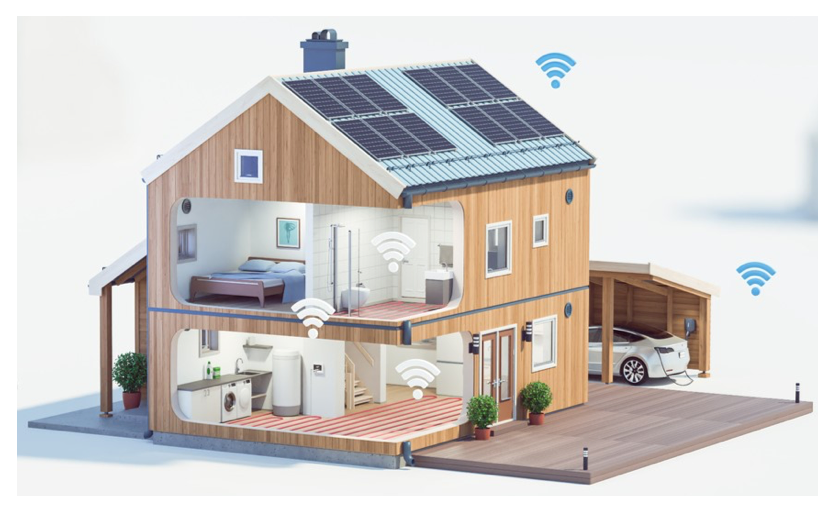
\includegraphics[width=1\textwidth,clip]{Figures/SmartHouse.eps}}

\tikzstyle{Sys_block} = [rectangle, draw, fill=none,  text width=3.cm, text centered, rounded corners, minimum height=4em,inner sep=2pt]
\tikzstyle{Obj_block} = [rectangle, draw, fill=myLightRed,  text width=2.7cm, text centered, rounded corners, minimum height=4em,inner sep=2pt]
\tikzstyle{Opt_block} = [rectangle, draw, fill=myLightGreen,  text width=3cm,  text centered, rounded corners]
\tikzstyle{ID_block} = [rectangle, draw, fill=myLightBlue,  text width=3cm, text centered, rounded corners]    
\tikzstyle{line} = [draw, -latex']

\begin{tikzpicture}[->,>=stealth']

\node [Sys_block] (sys0) {\Sys};

\node [ID_block, left of=sys0, node distance = 5cm] (ID0) {
 \begin{minipage}[c]{3cm}
\textbf{AI model} e.g.
\begin{align*}
\hat{\vect{s}}_{+} \sim \rho_{\vect{\theta}}\left(\cdot\,|\,\vect{s},\vect{a}\right)
\end{align*}
\vspace{-.75cm}
\flushright fitting data $\rho$
\end{minipage}
 };


 
 \node [Opt_block, below of=ID0, node distance = 2.7cm] (opt0) {
 \begin{minipage}[c]{3cm}
 \center
\textbf{Policy}\\
 \vspace{-0.6cm}
\begin{align*}
\vect\pi_{\vect\theta}(\vect{s})
\end{align*}
 \vspace{-0.5cm}\\
optimal for AI model 
\end{minipage}
 };
 
 \node [Obj_block, left of=opt0, node distance = 4cm] (Obj0) {
 \begin{minipage}[c]{2.7cm}
\textbf{Objective}
\vspace{-.5cm}\\
\begin{align*}
L\left(\vect s,\vect a\right)
\end{align*}
\vspace{-1.25cm}\\
\flushright possibly unbounded
\end{minipage}
 };
 
 \path 
 (sys0) edge  node[anchor=center,xshift=-.5em] {
  \begin{minipage}[c]{1cm}
  \center
 Data\\ knowledge
 \end{minipage}} (ID0)
 (ID0) edge[bend left=20]  node[anchor=west] {Predictions} (opt0)
 (opt0) edge[bend left=20]  node[anchor=east] {Actions} (ID0)
 (opt0) edge[bend right=20]  node[anchor=west,xshift=1em] {Policy} (sys0)
 (Obj0) edge  node[anchor=south] {Cost} (opt0)
 ;
\end{tikzpicture}

\textbf{Learning model $\rho_{\vect{\theta}}$ should aim at identifying 
}
\begin{align}
\label{eq:Jmin}
\vect{\theta}^\star =\argmin_{\vect{\theta} }\,J\left(\vect\pi_{\vect{\theta} }\right)
\end{align}
\vspace{-.6cm}
\visible<2->{
\begin{itemize}
\item Closed-loop performance $J$ is intricate ($\vect\theta\,\rightarrow\,$simulations$\,\rightarrow\,$policy$\,\rightarrow\,$real system)
\item \visible<3->{$\nabla_{\vect\theta}J\left(\vect\pi_{\vect\theta}\right)$ is to be estimated from data, i.e. data hungry, noisy, possible biases}
\item \visible<4->{\eqref{eq:Jmin} is in general different than model fitting, i.e. no loss function does  \eqref{eq:Jmin}}
\end{itemize}
}


\end{frame}




\begin{frame}{\normalsize Optimal AI models for Decision - A Paradigm Shift}
\footnotesize

\newcommand{\Sys}{\vspace{-0.25cm}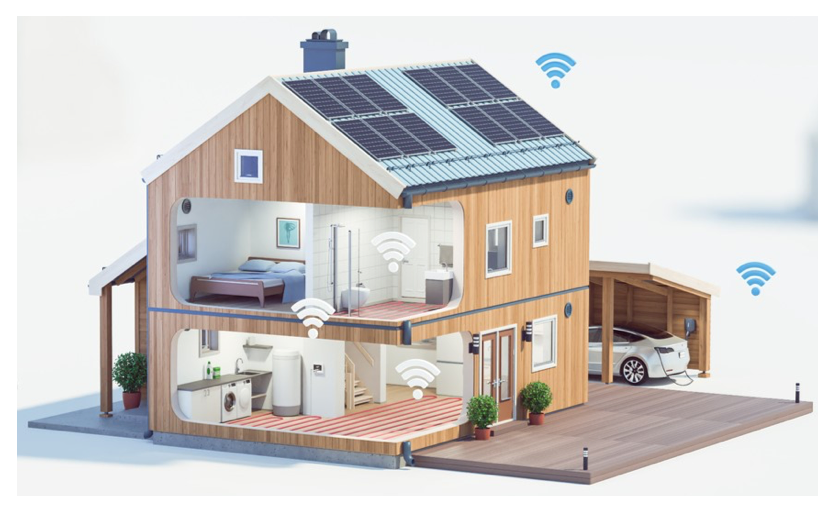
\includegraphics[width=1\textwidth,clip]{Figures/SmartHouse.eps}}

\tikzstyle{Sys_block} = [rectangle, draw, fill=none,  text width=3.cm, text centered, rounded corners, minimum height=4em,inner sep=2pt]
\tikzstyle{Obj_block} = [rectangle, draw, fill=myLightRed,  text width=2.7cm, text centered, rounded corners, minimum height=4em,inner sep=2pt]
\tikzstyle{Opt_block} = [rectangle, draw, fill=myLightGreen,  text width=3cm,  text centered, rounded corners]
\tikzstyle{ID_block} = [rectangle, draw, fill=myLightBlue,  text width=3cm, text centered, rounded corners]    
\tikzstyle{line} = [draw, -latex']

\begin{tikzpicture}[->,>=stealth']

\node [Sys_block] (sys0) {\Sys};

\node [ID_block, left of=sys0, node distance = 5cm] (ID0) {
 \begin{minipage}[c]{3cm}
\textbf{AI model} 
\begin{align*}
\hat{\vect{s}}_{+} \sim \rho_{\vect{\theta}}\left(\cdot\,|\,\vect{s},\vect{a}\right)
\end{align*}
\vspace{-.75cm}
 \visible<1-3>{\flushright fitting data $\rho$}
\end{minipage}
 };


 
 \node [Opt_block, below of=ID0, node distance = 3cm] (opt0) {
 \begin{minipage}[c]{3cm}
 \center
\textbf{Policy}
 \vspace{-0.1cm}
\begin{align*}
\vect\pi_{\vect \theta}(\vect{s})
\end{align*}
optimal for AI model
\end{minipage}
 };
 
 \node [Obj_block, left of=opt0, node distance = 4cm] (Obj0) {
 \begin{minipage}[c]{2.7cm}
\textbf{Objective}
\vspace{-.5cm}\\
\begin{overlayarea}{\textwidth}{0.1\textheight}
\only<1-2>{
\begin{align*}
L\left(\vect s,\vect a\right)
\end{align*}
}
\only<3->{
\begin{align*}
L_{\vect\theta}\left(\vect s,\vect a\right)
\end{align*}
}
\end{overlayarea}
\flushright possibly unbounded
\end{minipage}
 };
 
 \path 
 (sys0) edge  node[anchor=center,xshift=-.5em] {
  \begin{minipage}[c]{1cm}
  \center
 Data\\ knowledge
 \end{minipage}} (ID0)
 (ID0) edge[bend left=20]  node[anchor=west] {Predictions} (opt0)
 (opt0) edge[bend left=20]  node[anchor=east] {Actions} (ID0)
 (opt0) edge[bend right=20]  node[anchor=west,xshift=1em] {Policy} (sys0)
 (Obj0) edge  node[anchor=south] {Cost} (opt0)
 ;
 

 \visible<2->{\draw[blue,thick] ($(ID0.north east)+(+0.15,0.15)$)  rectangle ($(Obj0.south west)+(-0.15,-0.3)$);}
 
 
\end{tikzpicture}


\begin{overlayarea}{\textwidth}{0.25\textheight}



\only<2-4>{
\begin{itemize}
\item  The model is not $ \rho_{\vect{\theta}}$, it is the entire \textcolor{blue}{``decision-making box"}
\item  \visible<3->{The model includes objective $L_{\vect \theta}$ used to build the policy$^\star$}
\item  \visible<4->{Best model $\rho_{\vect\theta}$ should \textit{not necessarily} represent the data in a ``classical sense"}
\end{itemize}
\vspace{.5cm}
\visible<3->{\scriptsize $^\star$ policy performance on real system still assessed via $L$}
}

\only<5->{
\begin{alertblock}{}
\center
\textbf{Theorem}: under some (technical) assumptions, there is a $L_{\vect \theta}$ such that $\vect\pi_{\vect \theta}=\vect\pi_\star$, even if $ \rho_{\vect{\theta}}$ does not represent real world $\rho$ correctly
\end{alertblock}
}

\end{overlayarea}


\end{frame}







\begin{frame}{\normalsize How to use this more generally? RL over Policy Training}
\footnotesize

\newcommand{\Sys}{\vspace{-0.25cm}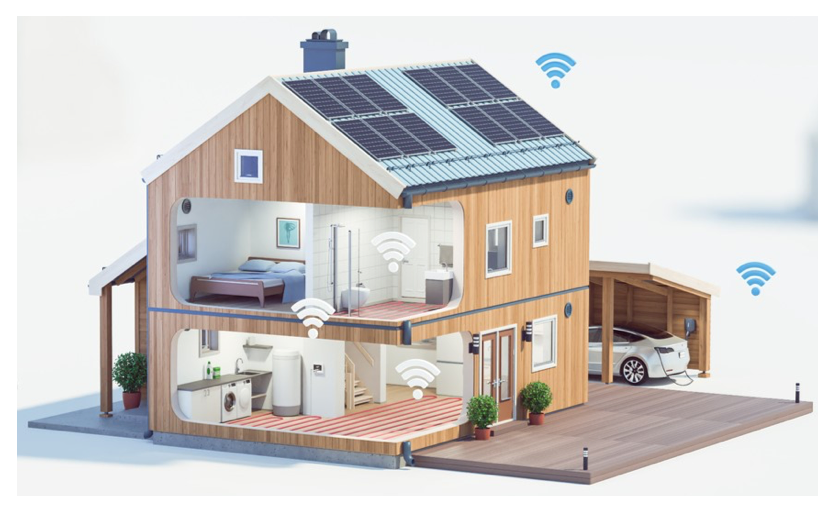
\includegraphics[width=1\textwidth,clip]{Figures/SmartHouse.eps}}

\tikzstyle{Sys_block} = [rectangle, draw, fill=none,  text width=3.cm, text centered, rounded corners, minimum height=4em,inner sep=2pt]
\tikzstyle{Obj_block} = [rectangle, draw, fill=myLightRed,  text width=2.7cm, text centered, rounded corners, minimum height=4em,inner sep=2pt]
\tikzstyle{Opt_block} = [rectangle, draw, fill=myLightGreen,  text width=3cm,  text centered, rounded corners]
\tikzstyle{ID_block} = [rectangle, draw, fill=myLightBlue,  text width=3cm, text centered, rounded corners]    

\tikzstyle{RL_block} = [rectangle, draw, fill=none,  text width=3.cm, text centered, rounded corners, minimum height=4em,inner sep=2pt]

\tikzstyle{line} = [draw, -latex']

\begin{tikzpicture}[->,>=stealth']

\node [Sys_block] (sys0) {\Sys};

\node [ID_block, left of=sys0, node distance = 5cm] (ID0) {
 \begin{minipage}[c]{3cm}
\textbf{AI model} 
 \vspace{-0.2cm}
\begin{align*}
\hat{\vect{s}}_{+} \sim \rho_{\vect{\theta}}\left(\cdot\,|\,\vect{s},\vect{a}\right)
\end{align*}
%\vspace{-.75cm}
% \visible<1-4>{\flushright fitting data}
\end{minipage}
 };

\visible<2->{
\node [RL_block, above of=ID0, node distance = 2cm] (RL0) {
 \begin{minipage}[c]{3cm}
\textbf{RL} 
\vspace{-.1cm} 
\begin{align*}
\Delta\vect\theta = \alpha\nabla_{\vect\theta} J\left(\vect\pi_{\vect \theta}\right)
\end{align*}
\vspace{-.85cm}
\flushright from data
\end{minipage}
 };}

 
 \node [Opt_block, below of=ID0, node distance = 2.0cm] (opt0) {
 \begin{minipage}[c]{3cm}
 \center
\textbf{Policy}
 \vspace{-0.2cm}
\begin{align*}
\vect\pi_{\vect \theta}(\vect{s})
\end{align*}
% \vspace{-0.25cm}\\
optimal for AI model
\end{minipage}
 };
 
 \node [Obj_block, left of=opt0, node distance = 4cm] (Obj0) {
 \begin{minipage}[c]{2.7cm}
\textbf{In-Sim Objective}
\vspace{-.5cm}\\
\begin{align*}
L_{\vect \theta}\left(\vect s,\vect a\right)
\end{align*}
\end{minipage}
 };
 
  \visible<2->{
  \node [Obj_block, left of=RL0, node distance = 4cm] (Obj1) {
 \begin{minipage}[c]{2.7cm}
\textbf{In-Real Objective}
\vspace{-.5cm}\\
\begin{align*}
L\left(\vect s,\vect a\right)
\end{align*}
\end{minipage}
 };}
 
 \path 
 (sys0) edge  node[anchor=center,xshift=-.5em] {
  \begin{minipage}[c]{1cm}
  \center
 Data\\ knowledge
 \end{minipage}} (ID0)
 (ID0) edge[bend left=20]  node[anchor=west] {Predictions} (opt0)
 (opt0) edge[bend left=20]  node[anchor=east] {Actions} (ID0)
 (opt0) edge[bend right=20]  node[anchor=west,xshift=1em] {Policy} (sys0)
 (Obj0) edge  node[anchor=south] {Cost} (opt0)
 ;
 
 \visible<2->{
 \path   (sys0) edge[bend right=20]  node[anchor=south west] {
  \begin{minipage}[c]{1cm}
  \center
 Data\\ knowledge
 \end{minipage}} (RL0)
   (RL0) edge[bend right=20]  node[anchor=south east] {$\Delta\vect\theta$} (Obj0)
  (RL0) edge  node[anchor=west] {$\Delta\vect\theta$} (ID0)
   (Obj1) edge  node[anchor=south east] {} (RL0)
  ;}


\draw[blue,thick] ($(ID0.north east)+(+0.15,0.15)$)  rectangle ($(Obj0.south west)+(-0.15,-0.3)$);
 
 
\end{tikzpicture}
\vspace{.2cm}
\begin{overlayarea}{\textwidth}{0.25\textheight}
\only<3>{\textbf{Policy gradient}
$$\nabla_{\vect \theta}J(\vect\pi_{\vect\theta}) = \mathbb E\left[ \nabla_{\vect \theta}\vect\pi_{\vect\theta} \nabla_{\vect a} Q^{\vect\pi_{\vect\theta}}\right]$$
\vspace{-.5cm}
\begin{itemize}
\item $Q^{\vect\pi_{\vect\theta}}$ is the critic, well-established RL tool
\item $\nabla_{\vect \theta}\vect\pi_{\vect\theta}$ requires differentiating the closed-loop simulation...
\end{itemize}
}
\only<4->{
\begin{block}{}
\center
\textbf{Difficulty}: computing $\nabla_{\vect \theta}\vect\pi_{\vect\theta}$ requires total differentiation through the simulation-based policy optimization process: \\
\textcolor{myBlue2}{$\vect\theta\,\rightarrow\,$simulations\textcolor{myRed2}{$\,\rightarrow\,$}optimal policy for $\rho_{\vect\theta}$}\\
Differentiating through policy optimization can be \textcolor{myRed2}{computationally heavy}
%\begin{itemize}
%\item ...
%\end{itemize}
%\textbf{Ingredients:}
%\begin{itemize}
%\item $Q^{\vect\pi_{\vect\theta}}$ is the ``critic", well-established RL methods to compute it
%\item $\nabla_{\vect \theta}\vect\pi_{\vect\theta}$ requires differentiating the optimal planning at every time step. Efficient methods are now available.
%\end{itemize}
\end{block}
}
\end{overlayarea}
\end{frame}

\begin{frame}{\normalsize Policy Differentiation}
\footnotesize
\begin{overlayarea}{\textwidth}{0.6\textheight}
\only<1-4>{
\textbf{Performance} for a stochastic policy $\pi_{\vect\nu}$, model MDP defined by $L_{\vect\theta},\, \hat\rho_{\vect\theta},\,\gamma$
\begin{align*}
\hat J_{\textcolor{myRed2}{\vect\theta}}\left(\pi_{\textcolor{myBlue3}{\vect\nu}}\right) = \mathbb E_{\hat\rho_{\textcolor{myRed2}{\vect\theta}}}\left[\,\left.\sum_{k=0}^N\gamma^k L_{\textcolor{myRed2}{\vect\theta}}\left(\vect s_k,\vect a_k\right)\,\right|\,\vect a_k\sim\pi_{\textcolor{myBlue3}{\vect\nu}}\left[\cdot|\vect s_k\right]\right]
\end{align*}
\vspace{-.8cm}
\visible<2->{
\flushleft \textbf{Policy} given by
\vspace{-.1cm}
\begin{align*}
\textcolor{myBlue3}{\vect\nu}^\star = \argmin_{\textcolor{myBlue3}{\vect\nu}}\, \hat J_{\textcolor{myRed2}{\vect\theta}}\left(\pi_{\textcolor{myBlue3}{\vect\nu}}\right) \qquad\text{or equivalently}\qquad \frac{\partial}{\partial \textcolor{myBlue3}{\vect\nu} } \hat J_{\textcolor{myRed2}{\vect\theta}}\left(\pi_{\textcolor{myBlue3}{\vect\nu}}\right)=0
\end{align*} }
\vspace{-.5cm}
\visible<3->{
\flushleft \textbf{Policy sensitivity}: if we change $\textcolor{myRed2}{\vect\theta}$ (cost $ L_{\textcolor{myRed2}{\vect\theta}}$ and simulation $\hat\rho_{\textcolor{myRed2}{\vect\theta}}$) how does $\pi_{\textcolor{myBlue3}{\vect\nu}}$ change?
\begin{align*}
\frac{\partial^2}{\partial \textcolor{myBlue3}{\vect\nu}^2} \hat J_{\textcolor{myRed2}{\vect\theta}}\left(\pi_{\textcolor{myBlue3}{\vect\nu}}\right)\underbrace{\frac{\mathrm d \pi_{\textcolor{myBlue3}{\vect\nu}}}{\mathrm d\textcolor{myRed2}{\vect\theta}}}_{=\nabla_{\vect\theta}\pi_{\vect\theta}}   + \frac{\partial^2}{\partial \textcolor{myBlue3}{\vect\nu}\partial \textcolor{myRed2}{\vect\theta} } \hat J_{\textcolor{myRed2}{\vect\theta}}\left(\pi_{\textcolor{myBlue3}{\vect\nu}}\right) = 0
\end{align*}}
}
\only<5>{
\begin{columns}
\column{0.5\textwidth}
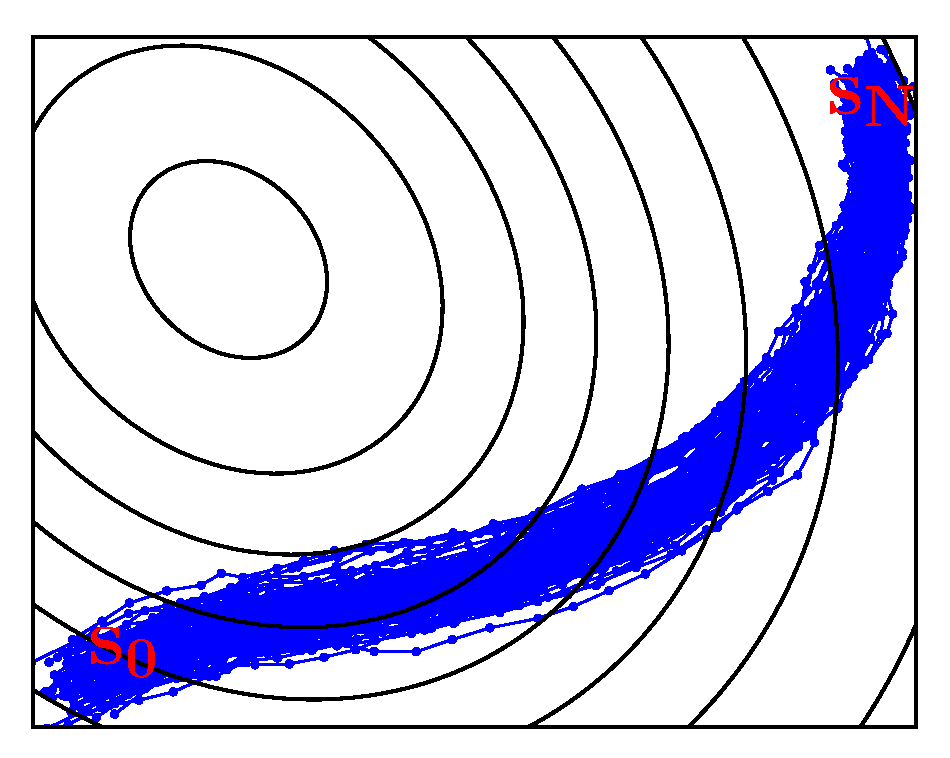
\includegraphics[width=1\textwidth,clip]{RLRL/ProbabilisticModel.eps}
\column{0.5\textwidth}
\begin{itemize}
\item Blue trajectories are realization of $\varphi$:
$$\vect s^i, \vect a^i \sim \varphi\left(\cdot,\cdot\right)$$
%\item ... with associated cost $$\sum_{k=0}^N\gamma^k L_{\textcolor{myRed2}{\vect\theta}}\left(\vect s_k,\vect a_k\right)$$
\item Sample-based evaluation ($n$ samples)
$$\hat J_{\textcolor{myRed2}{\vect\theta}}\left(\pi_{\textcolor{myBlue3}{\vect\nu}}\right) \approx \frac{1}{n}\sum_{k=i}^n\sum_{k=0}^N\gamma^k L_{\textcolor{myRed2}{\vect\theta}}\left(\vect s_k^i,\vect a_k^i\right)$$
\end{itemize}
\end{columns}
}
\end{overlayarea}
\vspace{-.5cm}
\visible<4->{
\flushleft \textbf{Simulation}: (with $\vect s\equiv \vect s_{0,\ldots,N}$ and $\vect a\equiv \vect a_{0,\ldots,N}$)
\begin{align*}
\hat J_{\textcolor{myRed2}{\vect\theta}}\left(\pi_{\textcolor{myBlue3}{\vect\nu}}\right) &=\int\sum_{k=0}^N\gamma^k L_{\textcolor{myRed2}{\vect\theta}}\left(\vect s_k,\vect a_k\right)\varphi\left(\vect s,\vect a\right)\mathrm d\vect s \mathrm d\vect a\\ \varphi\left(\vect s,\vect a\right) &= \rho_0\left[\vect s_0\right]\prod_{k=0}^{N-1}\hat\rho_{\textcolor{myRed2}{\vect\theta}}\left[\vect s_{k+1}|\vect s_k,\vect a_k\right]\prod_{k=0}^{N}\pi_{\textcolor{myBlue3}{\vect\nu}}\left[\vect a_k|\vect s_k\right]\qquad\text{(density of the simulation)}
\end{align*}}
\end{frame}

\begin{frame}{\normalsize Direct Simulation Differentiation}
\footnotesize
\begin{columns}
\column{0.6\textwidth}
\textbf{Simulation}
\begin{align*}
\hat J_{\textcolor{myRed2}{\vect\theta}}\left(\pi_{\textcolor{myBlue3}{\vect\nu}}\right) &=\int\sum_{k=0}^N\gamma^k L_{\textcolor{myRed2}{\vect\theta}}\left(\vect s_k,\vect a_k\right)\varphi\left(\vect s,\vect a\right)\mathrm d\vect s \mathrm d\vect a\\ \varphi\left(\vect s,\vect a\right) &= \rho_0\left[\vect s_0\right]\prod_{k=0}^{N-1}\hat\rho_{\textcolor{myRed2}{\vect\theta}}\left[\vect s_{k+1}|\vect s_k,\vect a_k\right]\prod_{k=0}^{N}\pi_{\textcolor{myBlue3}{\vect\nu}}\left[\vect a_k|\vect s_k\right]
\end{align*}
\column{0.4\textwidth}
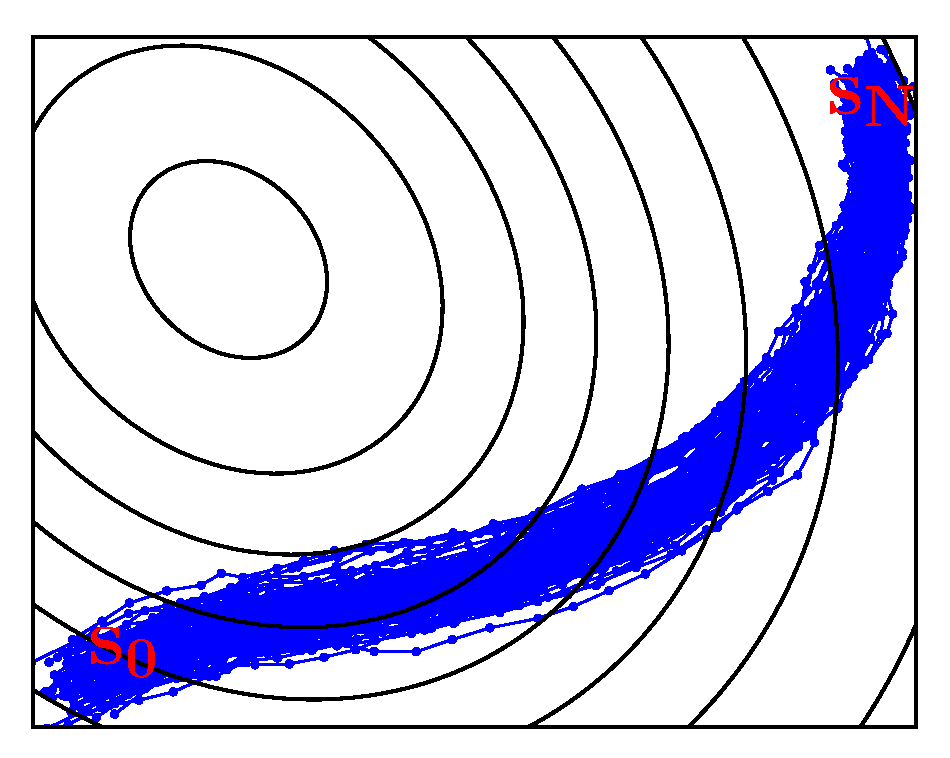
\includegraphics[width=1\textwidth,clip]{RLRL/ProbabilisticModel.eps}
\end{columns}

\vspace{-.25cm}
\visible<2->{
\flushleft\textbf{Direct Differentiation}:
\vspace{-.3cm}\\
\begin{overlayarea}{\textwidth}{0.2\textheight}
\only<2>{
\begin{align*}
\textcolor{myGreen2}{\partial} \hat J_{\textcolor{myRed2}{\vect\theta}}\left(\pi_{\textcolor{myBlue3}{\vect\nu}}\right) = \mathbb E_{\hat\rho_{\textcolor{myRed2}{\vect\theta}}}\left[\,\left.\sum_{k=0}^N\gamma^k\bigg(\textcolor{myGreen2}{\partial}L_{\textcolor{myRed2}{\vect\theta}}\left(\vect s_k,\vect a_k\right) + L_{\textcolor{myRed2}{\vect\theta}}\left(\vect s_k,\vect a_k\right)\textcolor{myGreen2}{\partial}\textcolor{myOrange2}{\log \varphi}\left(\vect s,\vect a\right)\bigg)\,\right|\,\vect a_k\sim\pi_{\textcolor{myBlue3}{\vect\nu}}\left[\cdot|\vect s_k\right]\right]
\end{align*}
can be evaluated from data}
\only<3->{
\begin{align*}
\textcolor{myGreen2}{\partial} \hat J_{\textcolor{myRed2}{\vect\theta}}\left(\pi_{\textcolor{myBlue3}{\vect\nu}}\right) \approx \frac{1}{n}\sum_{i=1}^n\sum_{k=0}^N\gamma^k\bigg(\textcolor{myGreen2}{\partial}L_{\textcolor{myRed2}{\vect\theta}}\left(\vect s_k^i,\vect a_k^i\right) + L_{\textcolor{myRed2}{\vect\theta}}\left(\vect s_k^i,\vect a_k^i\right)\textcolor{myGreen2}{\partial}\textcolor{myOrange2}{\log \varphi}\left(\vect s_k^i,\vect a_k^i\right)\bigg)
\end{align*}
}
\end{overlayarea}
}

\visible<4->{
\flushleft\textbf{Remarks}
\begin{itemize}
\item[$\checkmark$]  Second-order sensitivities are similar 
\item[$\checkmark$]  Simple and computationally very efficient
\item[$\checkmark$]  Can differentiate through discrete state and action sets
\item[\ding{56}] Sample-based estimations are very noisy 
\end{itemize}}



\end{frame}

\begin{frame}{\normalsize Critic-Based Differentiation}
\footnotesize\begin{columns}[t]
\column{0.65\textwidth}
\textbf{In-Sim Actor-critic} does
\begin{align*}
\nabla_{\textcolor{myBlue3}{\vect\nu}}\hat J_{\textcolor{myRed2}{\vect\theta}}\left(\pi_{\textcolor{myBlue3}{\vect\nu}}\right)=\mathbb E_{\tiny\begin{array}{l}\vect s\sim \rho_{\textcolor{myRed2}{\vect\theta}}\\\vect a\sim \pi_{\textcolor{myBlue3}{\vect\nu}}\end{array}}\left[\nabla_{\textcolor{myBlue3}{\vect\nu}}\log\pi_{\textcolor{myBlue3}{\vect\nu}}\left(\vect a|\vect s\right)A^{\vect \pi_{\textcolor{myBlue3}{\vect\nu}}}\left(\vect s, \vect a\right)\right]=0
\end{align*}
\begin{flushright} defines relationship $\pi_{\textcolor{myBlue3}{\vect\nu^\star}}$ with $\textcolor{myBlue3}{\vect\nu^\star}$ function of $\textcolor{myRed2}{\vect\theta}$\end{flushright}
\visible<2->{
\textbf{In-Real Actor-critic} evaluates
\begin{align*}
\nabla_{\textcolor{myRed2}{\vect\theta}}J\left(\pi_{\textcolor{myBlue3}{\vect\nu^\star}}\right)=\mathbb E_\text{Real World}\left[\nabla_{\textcolor{myRed2}{\vect\theta}}\log\pi_{\textcolor{myBlue3}{\vect\nu^\star}}\left(\vect a|\vect s\right)A^{\textcolor{myBlue3}{\vect\nu^\star}}\left(\vect s, \vect a\right)\right]
\end{align*}}
\visible<3->{where $\nabla_{\textcolor{myRed2}{\vect\theta}}\log\pi_{\textcolor{myBlue3}{\vect\nu^\star}}\left(\vect a|\vect s\right)$ requires $\frac{\mathrm d {\textcolor{myBlue3}{\vect\nu^\star}}}{\mathrm d\textcolor{myRed2}{\vect\theta}}  $}\\
\vspace{.5cm}
\visible<3->{
\textbf{Sensitivity}
\begin{align*}
\frac{\partial^2}{\partial \textcolor{myBlue3}{\vect\nu}^2} \hat J_{\textcolor{myRed2}{\vect\theta}}\left(\pi_{\textcolor{myBlue3}{\vect\nu^\star}}\right)\frac{\mathrm d {\textcolor{myBlue3}{\vect\nu^\star}}}{\mathrm d\textcolor{myRed2}{\vect\theta}}  + \frac{\partial^2}{\partial \textcolor{myBlue3}{\vect\nu}\partial \textcolor{myRed2}{\vect\theta} } \hat J_{\textcolor{myRed2}{\vect\theta}}\left(\pi_{\textcolor{myBlue3}{\vect\nu^\star}}\right) = 0
\end{align*}
}
\column{0.35\textwidth}
\vspace{-1cm}
\begin{figure}
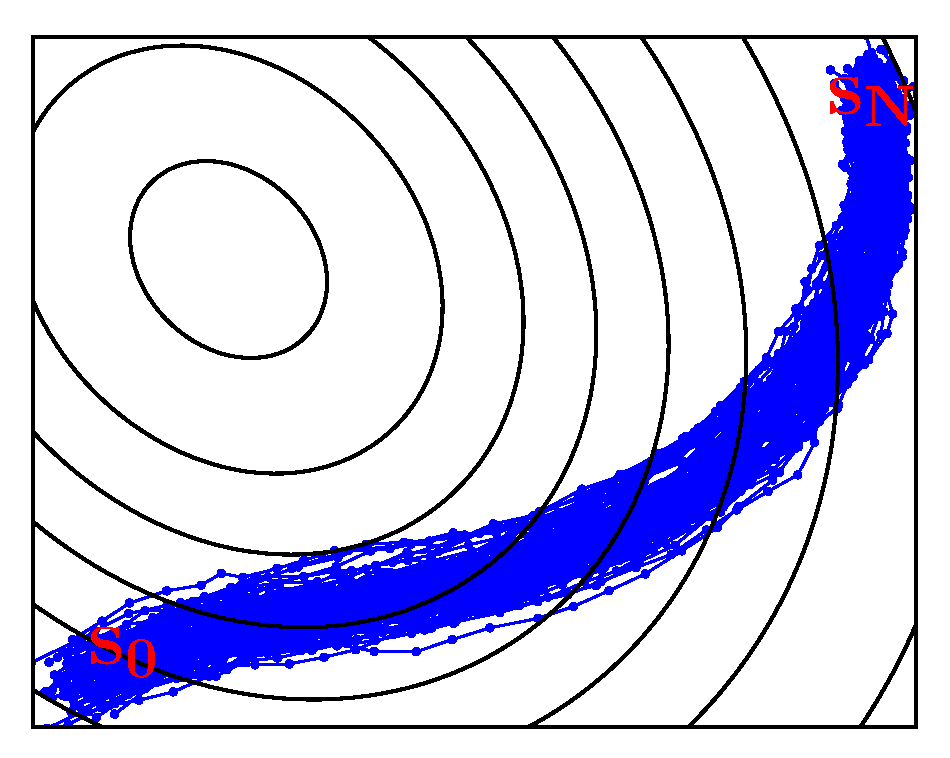
\includegraphics[width=1\textwidth,clip]{RLRL/ProbabilisticModel.eps}
\end{figure}
\end{columns}
\visible<4->{
\textbf{
Idea}: compute $\frac{\mathrm d {\textcolor{myBlue3}{\vect\nu^\star}}}{\mathrm d\textcolor{myRed2}{\vect\theta}}$ from differentiating the in-sim actor-critic w.r.t. $\frac{\partial}{\partial \textcolor{myBlue3}{\vect\nu}}$ and $\frac{\partial}{\partial \textcolor{myRed2}{\vect\theta} } $
}
\visible<5->{\center
\textbf{Proposed first algorithm to do that.\\Computationally heavy, but we have ``missed" some simplifications, testing further}
}
\end{frame}

\begin{frame}{\normalsize Example - In-Real RL over In-Sim RL}
\footnotesize
\center
\visible<2->{
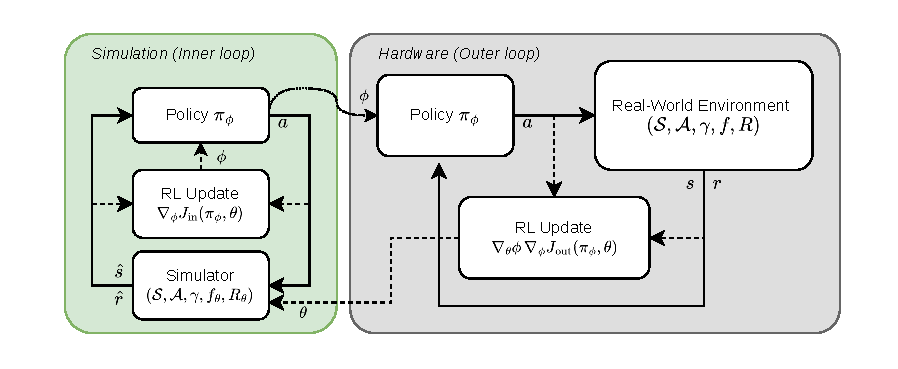
\includegraphics[width=0.8\textwidth,clip]{RLRL/rl_over_rl_overview.eps}}
\begin{columns}
\column{0.45\textwidth}
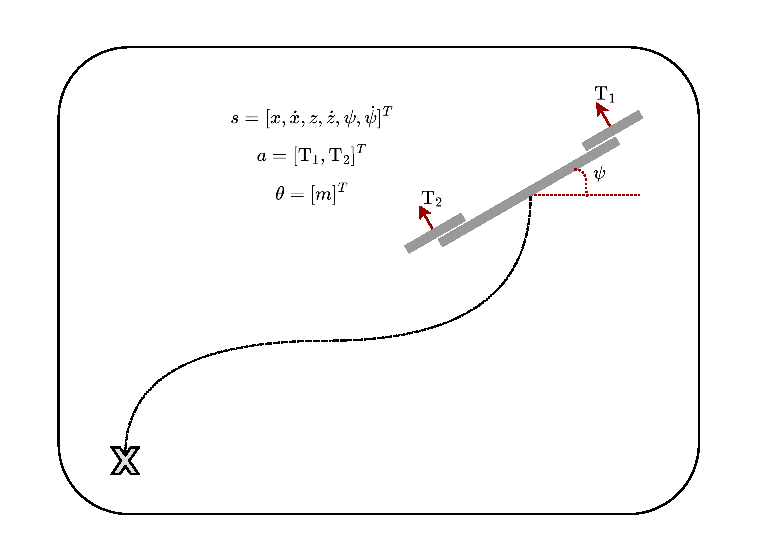
\includegraphics[width=1\textwidth,clip]{RLRL/quad2d_task.eps}
\column{0.55\textwidth}
\includegraphics<3->[width=1\textwidth,clip]{RLRL/perf_bi_ppo_quad2d.eps}
\end{columns}


\end{frame}


\begin{frame}{\textbf{Norwegian Center on AI for Decisions}}
\footnotesize
\vspace{-0.5cm}
\begin{columns}
\column{0.8\textwidth}
\column{0.2\textwidth}
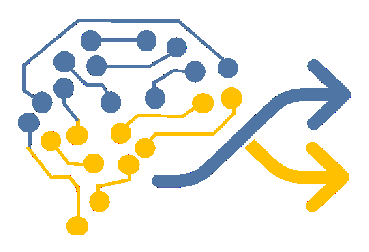
\includegraphics[width=.9\textwidth,clip]{Figures/AID.eps}
\end{columns}
\vspace{-0.75cm}
\begin{columns}
\column{0.35\textwidth}
\center
\textbf{Email}\\
\vspace{0.2cm}

\includegraphics[width=.6\textwidth,clip]{Email.eps}
\vspace{0.2cm}
\begin{itemize}
\item Start-up phase
\item Recruiting soon!
\item We can apply for funding to bring strong international postdocs
\end{itemize}
\vspace{0.6cm}
\begin{center}
{\Huge
Thank you!}
\end{center}


\column{0.65\textwidth}
\center

\includegraphics[width=1\textwidth,clip]{Figures/AID2.eps}
\end{columns}

%\center \footnotesize
%MPC-heavy... but new (and more general) publications are coming!

\end{frame}

\end{document}

